\documentclass[11pt]{article}
\usepackage[margin=1in]{geometry}
\usepackage[T1]{fontenc}
\usepackage{lmodern}
\usepackage{amsmath,amssymb,amsthm,mathtools,amscd}
\usepackage{booktabs,array,longtable,enumitem,microtype}
\usepackage{graphicx}
\usepackage{tikz}
\usetikzlibrary{arrows.meta,positioning,calc}
\usepackage{hyperref}
\hypersetup{
  hidelinks,
  pdftitle={Correspondence and Logical Matrices: A Typed Boolean Operator Calculus},
  pdfauthor={Brian Theory},
  pdfkeywords={Boolean algebra, formula-valued logical matrices, correspondence matrices, logical pairing, operator superposition, propositional logic, truth tensors}
}

\newtheorem{theorem}{Theorem}[section]
\newtheorem{lemma}[theorem]{Lemma}
\newtheorem{proposition}[theorem]{Proposition}
\newtheorem{corollary}[theorem]{Corollary}
\theoremstyle{definition}
\newtheorem{definition}[theorem]{Definition}
\newtheorem{example}[theorem]{Example}
\theoremstyle{remark}
\newtheorem{remark}[theorem]{Remark}

\newcommand{\B}{\mathbb B}
\newcommand{\F}{\mathbb F}
\newcommand{\cF}{\mathcal F}
\newcommand{\cC}{\mathcal C}
\newcommand{\cM}{\mathcal M}
\newcommand{\cO}{\mathcal O}
\newcommand{\cP}{\mathcal P}
\newcommand{\cT}{\mathcal T}
\newcommand{\GL}{\operatorname{GL}}
\newcommand{\wt}{\operatorname{wt}}
\newcommand{\rot}{\operatorname{rot}}
\newcommand{\vecop}{\operatorname{vec}}
\newcommand{\ANF}{\operatorname{ANF}}
\newcommand{\xor}{\mathbin{\Updownarrow}}
\newcommand{\bigxor}{\mathop{\Updownarrow}\displaylimits}
\newcommand{\landop}{\mathbin{\wedge}}
\newcommand{\true}{1}
\newcommand{\false}{0}
\newcommand{\Pair}{\operatorname{Pair}}
\newcommand{\Span}{\operatorname{span}}
\newcolumntype{L}[1]{>{\raggedright\arraybackslash}p{#1}}

\setlength{\emergencystretch}{3em}
\setlist[itemize]{leftmargin=1.6em}
\setlist[enumerate]{leftmargin=1.8em}

\title{Correspondence and Logical Matrices:\\A Typed Boolean Operator Calculus\\[0.4em]
\large Formula-valued logical matrices, valuation, pairing, and coherent operator superposition}
\author{Brian Theory}
\date{September 2026}

\begin{document}
\maketitle

\begin{abstract}
We develop a typed Boolean operator calculus centered on formula-valued logical matrices (LMs) and their relation to numeric correspondence matrices (CMs).  For a binary connective $\Theta$, the LM
\[
 [M_{X\Theta Y}]
 =\begin{bmatrix}
 X\Theta Y & X\Theta\neg Y\\
 \neg X\Theta Y & \neg X\Theta\neg Y
 \end{bmatrix}
\]
records the complete polarity orbit of the logical operands $X,Y$.  It admits the invertible Boolean-frame normal form
\[
 [M_{X\Theta Y}]=\mathsf S_X[\Theta]\mathsf S_Y,
 \qquad
 \mathsf S_X=\begin{bmatrix}X&\neg X\\ \neg X&X\end{bmatrix},
 \qquad \mathsf S_X^2=I,
\]
so valuation sends the symbolic operator to the corresponding numeric CM in its valued signed frame.  Logical pairing has the exact agreement-bit semantics
\[
 \langle A|[M_{X\Theta Y}]|B\rangle
 \equiv (A\Leftrightarrow X)\,\Theta\,(Y\Leftrightarrow B),
\]
and labelled basis pairings reconstruct the connective.

The central operation is Boolean superposition of aligned logical operators.  If an outer Boolean operation $g$ is applied pointwise to formula-valued LMs, the LM lift, valuation, common signed input-frame transport, and logical pairing all preserve the same operation.  The corresponding CM-level entrywise law is a valued corollary and has direct antecedents in truth-vector Boolean calculus; the focus here is the formula-valued LM architecture and the coherence of its symbolic, relational, and numeric semantics.  We extend the construction to arbitrary-arity logical tensors and rectangular correspondence maps, give conditional block constructions, and characterize conjunctive/XOR separability by ordinary $\F_2$ matrix rank.

The underlying truth-table, Boolean-algebra, group-action, and pointwise-composition ingredients are classical.  The paper therefore claims a unified formula-valued symbolic/numeric representation calculus and precise compatibility laws rather than a new underlying Boolean algebra.  No physical measurement interpretation, truth-table compression, or computational speedup is assumed.
\end{abstract}

\paragraph{Contribution and scope.}
The contribution claimed here is a typed synthesis: a formula-valued polarity lift, an explicit Boolean frame normal form, agreement-bit pairing, signed-frame transport, and coherence identities linking symbolic LMs to numeric CMs.  The constituent truth-table, Boolean-matrix, group-action, pointwise-composition, tensor-flattening, and rank mechanisms have substantial prior art, so the paper does not claim firstness for those ingredients.  Its mathematical claims are the stated representation identities and their integration into one frame-aware calculus.  The representation is exact rather than compressed, and no computational speedup or physical measurement interpretation is assumed.

\section{Introduction}

Every binary Boolean connective has four output values.  A truth table records those values as data; a correspondence matrix records them in a $2\times2$ array whose row and column axes are tied to declared operands.  The information content is unchanged, but the array can participate in an operator calculus.  True-first Boolean state vectors select entries; transposition exchanges operand axes; row and column reversals absorb input negations; output complement negates the connective; and compatible operators can be combined before any particular operands are evaluated.

A small alignment failure motivates making the frame part of the type.  The two occurrences in $(X\Rightarrow Y)\xor(Y\Rightarrow X)$ both use the local implication table.  XORing those two unlabelled arrays would therefore give zero.  In a common $(X,Y)$ frame, however, the second occurrence is $[\Rightarrow]^T$, and $[\Rightarrow]\,\widehat{\Updownarrow}\,[\Rightarrow]^T=[\Updownarrow]$, correctly yielding $X\xor Y$.  Section~\ref{sec:operatoronoperator} carries this example through the symbolic LM, valuation, and pairing layers.

The notation follows the author's original manuscript \cite{Droncheff2018}.  A Greek letter such as $\Theta$ denotes a logical operator variable, and $[\Theta]$ denotes the correspondence matrix representing that operator.  Thus $\Theta=\Leftrightarrow$ is a connective while
\[
 [\Leftrightarrow]=\begin{bmatrix}1&0\\0&1\end{bmatrix}
\]
is its CM.  When arbitrary arity is required we use ordinary function notation $f:\B^n\to\B$; for a binary named connective, $f_\Theta(x,y)=x\Theta y$.  This separates the connective from its matrix representation without introducing a second unrelated symbol for the binary CM.

Throughout the paper, uppercase symbols such as $X,Y,A,B$ denote logical operands or formulas, while lowercase symbols such as $x,y,a,b,c,d$ denote Boolean values, assignments, or scalar coefficients.  The uppercase operands need not be atomic propositional variables: they may be arbitrary formulas.  The present theory nevertheless keeps LM entries in the Boolean formula algebra; an enrichment in which the operands or entries are themselves matrix-valued operators is a separate extension and is not assumed here.

Earlier correspondence-matrix work introduced the terminology and several constructions used here, including binary CMs, formula-valued LMs, matrix transformations, logical pairing, and preliminary higher-dimensional examples \cite{Droncheff2018}.  The present paper restates only the mathematically supported parts in an explicit type system.  In particular, the former arithmetic-modulo and measurement analogies are not premises of the calculus; higher-dimensional objects are treated as $2^n$-entry truth tensors with declared matrix flattenings.

The central structural claim is not that truth tables, Boolean matrices, tensor flattenings, or pointwise composition are new.  The distinctive focus is the formula-valued LM layer and the compatibility of its semantics with the numeric CM layer.  The architecture organizes several levels of the same Boolean function:
\begin{enumerate}
  \item \textbf{formula-valued logical operators:} for example $[M_{X\lor Y}]$, whose four entries are $X\lor Y$, $X\lor\neg Y$, $\neg X\lor Y$, and $\neg X\lor\neg Y$;
  \item \textbf{valuation to numeric correspondence operators:} a valuation sends an LM to a four-bit CM such as $[\Rightarrow]=\bigl[\begin{smallmatrix}1&0\\1&1\end{smallmatrix}\bigr]$, with the valued operand polarities recorded by row/column reversals;
  \item \textbf{logical pairing:} contraction of a formula-valued LM against formula states, producing an exact relationship formula rather than merely selecting a stored bit;
  \item \textbf{LM operator superposition:} aligned formula-valued logical operators themselves become operands of another Boolean operation, producing a new LM; the familiar CM entrywise law is its valued numeric image;
  \item \textbf{signed-frame actions:} input permutations and polarity changes realized coherently as symbolic substitutions and numeric matrix/tensor reindexings; and
  \item \textbf{higher-arity logical tensors and correspondence maps:} the same construction extends to $2^n$ symbolic polarity slots and to typed rectangular flattenings.
\end{enumerate}
The point of the calculus is that these maps and operations are linked by commuting identities rather than merely listed side by side.

A further goal is to make the binary construction scale cleanly.  An $n$-variable function has a canonical $2\times\cdots\times2$ correspondence tensor.  A formula-valued version is its symbolic polarity orbit.  A row/column bipartition of $p$ and $q$ variables reshapes the tensor into a $2^p\times2^q$ correspondence map.  Square flattenings are endomorphisms; rectangular flattenings are linear maps between different Boolean state spaces.  Both still support a typed bra--matrix--ket contraction.

Matrix representations of logic have extensive antecedents.  Boolean matrix methods predate CMs \cite{Edwards1972}; matrix and vector logic treat logical connectives as operators \cite{Stern1988,Mizraji1992,Mizraji2008}; semi-tensor-product methods use logical structure matrices \cite{ChengQi2010,ZhaoSTP}; and explicit XOR--AND Boolean matrix calculi also exist \cite{Cheng2011}.  Most importantly for the raw numeric operator-on-operator law, Cheng, Zhao, and Xu state that if two Boolean functions of the same ordered variables have truth vectors $m_f,m_g$, then the truth vector of $f\,\Phi\,g$ is obtained by applying the outer logical operator $\Phi$ entrywise to $m_f,m_g$ \cite[Prop.~3.3]{Cheng2011}.  Under a $2\times2$ reshape this is the numeric same-frame identity used here.  In the inspected Cheng source, however, the relevant construction is expressed in truth-vector/Boolean-matrix language; we did not locate a formula-valued LM polarity lift, the present logical-pairing identity, or a bra--matrix--ket semantic layer there.  Accordingly, pointwise combination of aligned numeric truth values is not claimed as new; the present paper centers the formula-valued LM architecture and the way valuation, pairing, and typed frame transport preserve the same operation.

Bricken's internally dated March 1997 notes are another close antecedent: they arrange the sixteen binary Boolean relations as $2\times2$ matrices, use Boolean matrix algebra, explicitly evaluate logical operators in bra--matrix--ket form $\langle x|B|y\rangle$, and treat logical matrices as operands of matrix operations \cite{Bricken1997}.  The original public-release date and peer-reviewed status of that technical note should not be inferred from the current website alone.  Thus neither Dirac-style notation, $2\times2$ logical matrices, nor the broad idea that matrices representing logic can themselves be manipulated is claimed as new.  NPN transformations and packed truth-function manipulation are likewise standard in logic synthesis \cite{Mishchenko2006,Zhou2019}.

Eigenlogic supplies a second important boundary.  Its published treatment represents logical propositions by commuting projection operators whose truth values are eigenvalues and whose canonical interpretations are eigenvectors \cite{Toffano2020,DuboisToffano2016}.  The CM/LM contribution pursued here is different and narrower: formula-valued polarity operators, their valuation to numeric CMs, exact logical pairing, typed frame alignment, and a coherence law showing that Boolean operations on operators are respected by valuation, frame changes, and pairing.  The abstract orbit embedding and polarity-equivariance facts are standard group-action structure and are used for characterization rather than historical priority.

\section{Boolean scalar algebra and correspondence operators}
\label{sec:cm}

\subsection{Three distinct compositions}

The same finite arrays participate in several different operations, and the paper keeps them explicitly separate.
\begin{enumerate}
\item \emph{XOR--AND matrix product} $AB$ contracts an intermediate matrix index over $\F_2$.
\item \emph{Pointwise Boolean operator superposition} $A\,\widehat\Phi\,B$ applies an outer Boolean connective $\Phi$ to corresponding entries of two operators in the same declared frame.
\item \emph{Boolean-function superposition} $h=g(f_1,\ldots,f_m)$ substitutes the outputs of Boolean functions into an outer Boolean function $g$.
\end{enumerate}
The representation theorems below realize the third operation by the second when the operators are aligned; they do not identify either of those operations with ordinary matrix multiplication.  A separate matched-intermediate-frame theorem later explains when the first operation also transports cleanly through the LM representation.

\subsection{States, one-hot selection, and binary CMs}

Let $\B=\{0,1\}$ and regard it as $\F_2$ when addition and multiplication are used.  Addition is XOR, written $\xor$, and multiplication is conjunction.  The nonstandard XOR glyph is intentional: in the declared true-first CM frame, the XOR matrix is the literal quarter-turn rotation of the XNOR matrix,
\begin{equation}
 [\Leftrightarrow]=\begin{bmatrix}1&0\\0&1\end{bmatrix},\qquad
 [\Updownarrow]=\begin{bmatrix}0&1\\1&0\end{bmatrix}
 =\rot\!\left([\Leftrightarrow]\right).
 \label{eq:xorrotationmotivation}
\end{equation}
The notation is paper-specific rather than a claim of standard usage.  Logical equivalence of formulas is written $\equiv$; the connective itself is written $\Leftrightarrow$.

For a bit $x\in\B$, define the true-first state
\begin{equation}
 |x\rangle=\begin{bmatrix}x\\ \neg x\end{bmatrix},
 \qquad
 \langle x|=\begin{bmatrix}x&\neg x\end{bmatrix}.
 \label{eq:state}
\end{equation}
These are \emph{one-hot} states: exactly one component is $1$.  Thus $|1\rangle=(1,0)^T$ and $|0\rangle=(0,1)^T$.  Bra--ket notation is used only as compact row/map/column notation in a Boolean algebra; no Hilbert-space or physical interpretation is assumed.

Let $\Theta$ be a binary logical operator variable.  Its correspondence matrix is
\begin{equation}
 [\Theta]:=
 \begin{bmatrix}
 1\Theta1&1\Theta0\\
 0\Theta1&0\Theta0
 \end{bmatrix}
 =\begin{bmatrix}\Theta_{11}&\Theta_{10}\\\Theta_{01}&\Theta_{00}\end{bmatrix}.
 \label{eq:binarycm}
\end{equation}
The brackets are part of the notation: $\Theta$ is the logical operator, while $[\Theta]$ is its CM representation.  For general functional notation, write $f_\Theta(x,y)=x\Theta y$.

\begin{proposition}[Unique binary representation]
Once the operand axes and true-first order are fixed, $\Theta\mapsto[\Theta]$ is a bijection between the sixteen binary Boolean operators and the sixteen matrices in $\B^{2\times2}$.
\end{proposition}
\begin{proof}
A binary operator is determined by its four values on $(1,1),(1,0),(0,1),(0,0)$, exactly the four entries of $[\Theta]$.
\end{proof}

For any $C\in\B^{2\times2}$ define the XOR--AND contraction
\begin{equation}
 E_C(x,y)=\langle x|C|y\rangle
 =\bigxor_{r,s\in\{1,0\}}
 \chi_x(r)\land C_{rs}\land\chi_y(s),
 \label{eq:contraction}
\end{equation}
where $\chi_x(r)=1$ exactly when $r=x$.

\begin{proposition}[CM selection]
\label{prop:cmselection}
For every binary operator $\Theta$ and $x,y\in\B$,
\[
 \langle x|[\Theta]|y\rangle=x\Theta y.
\]
\end{proposition}
\begin{proof}
Both states are one-hot.  Every term in \eqref{eq:contraction} vanishes except the term indexed by $(r,s)=(x,y)$.
\end{proof}

\begin{remark}[Why XOR--AND rather than OR--AND?]
For one-hot basis states, XOR--AND and OR--AND selection return the same selected coefficient because at most one product term can be nonzero.  For example, if $[\Theta]=\bigl[\begin{smallmatrix}a&b\\c&d\end{smallmatrix}\bigr]$, then $\langle1|[\Theta]|0\rangle=b$ under either reduction.  This observation already appears in the historical manuscript \cite{Droncheff2018}.

The two algebras are not interchangeable in general.  With $u=(1,1)$ and $v=(1,1)^T$,
\[
 u\cdot_{\mathrm{XOR/AND}}v=1\xor1=0,
 \qquad
 u\cdot_{\mathrm{OR/AND}}v=1\lor1=1.
\]
Thus arbitrary vector or matrix multiplication can differ as soon as more than one term survives.  XOR is retained because it gives the $\F_2$ coefficient algebra, coefficient-space linearity, cancellation, and a single convention shared by the numeric and symbolic calculus.  Short-circuit evaluation of the logical connective OR is a separate implementation issue and does not justify replacing the contraction algebra globally.
\end{remark}

\subsection{Basis decomposition and Boolean closure at the coefficient level}

Let $E_{rs}=|r\rangle\langle s|$ for $r,s\in\{1,0\}$.  These four one-feature matrices form the standard basis of $\F_2^{2\times2}$.
\begin{proposition}[CM basis decomposition]
Every binary CM has the unique expansion
\begin{equation}
 [\Theta]=\bigxor_{r,s\in\{1,0\}}\Theta_{rs}E_{rs}.
 \label{eq:basisdecomp}
\end{equation}
\end{proposition}
This recovers one of the original CM constructions in a conventional vector-space form: a connective is the XOR sum of exactly those minterm positions on which it is true \cite{Droncheff2018}.

The contraction is linear in the coefficients of $[\Theta]$ over $\F_2$ for fixed states.  This does not imply that the represented Boolean function is affine in its logical inputs.

\subsection{Operand frames and the internal swap matrix}

A CM occurrence is typed by its operand frame: row expression, column expression, input polarities, and truth-state order.  Define the transformed connectives by their truth functions
\[
 \Theta^\tau(x,y):=y\Theta x,\qquad
 \Theta^{\neg L}(x,y):=(\neg x)\Theta y,\qquad
 \Theta^{\neg R}(x,y):=x\Theta(\neg y).
\]
Then
\begin{equation}
 [\Theta^\tau]=[\Theta]^T,\qquad
 [\Theta^{\neg L}]=[\Updownarrow][\Theta],\qquad
 [\Theta^{\neg R}]=[\Theta][\Updownarrow].
 \label{eq:binaryframe}
\end{equation}
The matrix products in \eqref{eq:binaryframe} are XOR--AND products.  Here $[\Updownarrow]$ plays two compatible roles: as the CM of the XOR connective and, under matrix multiplication, as the two-state permutation matrix that exchanges true and false.  This removes the need to introduce an unrelated symbol $P$ or $S$ for the same $2\times2$ array.

Output complement is entrywise.  If $J$ is the all-ones $2\times2$ matrix, then
\begin{equation}
 [\neg\Theta]=J\xor[\Theta].
 \label{eq:outputcomplement}
\end{equation}

\subsection{Support order and Boolean difference}

The original manuscript used the language of operator containment and ``quotienting.''  The sound part is most cleanly stated as a support order.  For CMs $A,B\in\B^{2\times2}$ write
\[
 A\preceq B
 \quad\Longleftrightarrow\quad
 A_{rs}\le B_{rs}\text{ for every }r,s,
\]
so $\operatorname{supp}(A)\subseteq\operatorname{supp}(B)$.  Define the Boolean support difference
\begin{equation}
 B\setminus A:=B\land\neg A
 \label{eq:supportdifference}
\end{equation}
entrywise.  For example,
\[
 [\lor]\setminus[\land]=[\Updownarrow].
\]
This is ordinary Boolean set difference on truth support, not arithmetic remainder or modulo.  It is useful for decompositions and comparisons, but it is not a new scalar operation.

\begin{figure}[ht]
\centering
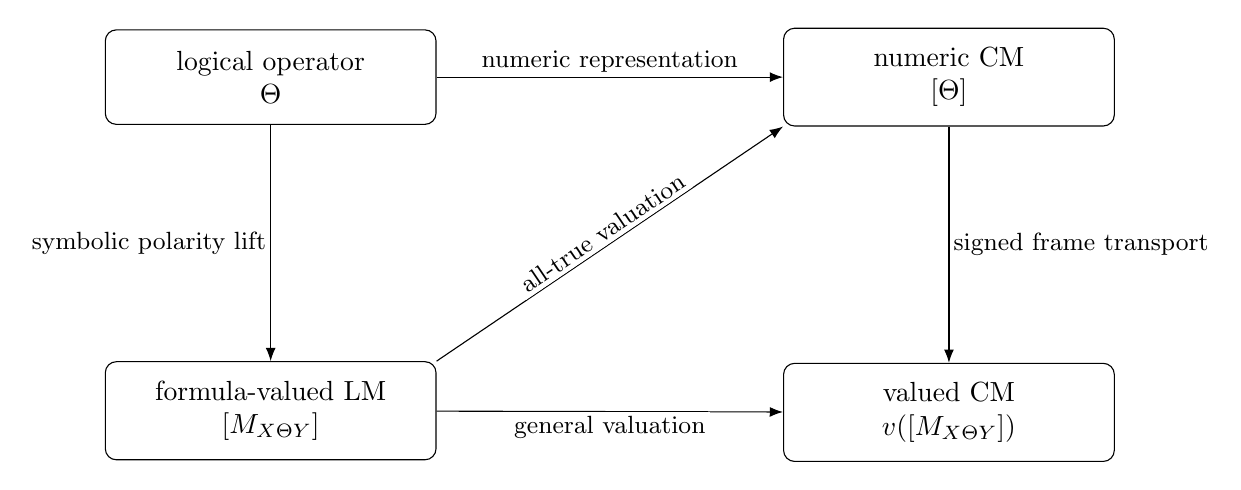
\begin{tikzpicture}[>=Latex,
  box/.style={draw,rounded corners,align=center,minimum width=42mm,minimum height=12mm,inner sep=7pt},
  lab/.style={fill=white,inner sep=1.5pt,align=center,font=\small}]
\node (op) [box] {logical operator\\$\Theta$};
\node (cm) [box,right=44mm of op] {numeric CM\\$[\Theta]$};
\node (lm) [box,below=30mm of op] {formula-valued LM\\$[M_{X\Theta Y}]$};
\node (val) [box,below=30mm of cm] {valued CM\\$v([M_{X\Theta Y}])$};
\draw[->] (op) -- node[lab,above]{numeric representation} (cm);
\draw[->] (op) -- node[lab,left]{symbolic polarity lift} (lm);
\draw[->] (lm) -- node[lab,below]{general valuation} (val);
\draw[->] (cm) -- node[lab,right]{signed frame transport} (val);
\draw[->] (lm.north east) -- node[lab,sloped,above]{all-true valuation} (cm.south west);
\end{tikzpicture}
\caption{Binary CM/LM architecture.  The connective $\Theta$, its numeric matrix $[\Theta]$, and its formula-valued LM are distinct typed objects.  For free reference generators the all-true valuation returns $[\Theta]$; arbitrary valuations return signed-frame versions.}
\label{fig:binaryarchitecture}
\end{figure}

\section{Formula-valued logical matrices}
\label{sec:lm}

\subsection{Binary symbolic lift}

Let $\cF$ be the Boolean algebra of formulas modulo logical equivalence.  Unless stated otherwise, $X$ and $Y$ in the defining LM are distinct free reference generators.  The same formulas may later be specialized to compound operands; in that case general valuation remains valid, but an ``all-true'' valuation exists only when those substituted references are jointly satisfiable.  For a formula $A$ and polarity bit $b\in\B$, write
\begin{equation}
 A^{\langle b\rangle}=\begin{cases}A,&b=1,\\\neg A,&b=0.\end{cases}
 \label{eq:polarity}
\end{equation}
For a binary operator $\Theta$, define the formula-valued logical matrix
\begin{equation}
 [M_{X\Theta Y}]:=
 \begin{bmatrix}
 X\Theta Y&X\Theta\neg Y\\
 \neg X\Theta Y&\neg X\Theta\neg Y
 \end{bmatrix}.
 \label{eq:binarylm}
\end{equation}
Its entries are formulas, not numeric coefficients.  For example,
\[
 [M_{X\lor Y}]=
 \begin{bmatrix}
 X\lor Y&X\lor\neg Y\\
 \neg X\lor Y&\neg X\lor\neg Y
 \end{bmatrix}.
\]
Thus the LM packages the complete polarity orbit of one reference formula.

\subsection{Formula-valued frame normal form}

There is a compact matrix factorization behind the four displayed formulas.  Whenever juxtaposition of formula-valued matrices is used in this paper, it denotes XOR--AND matrix multiplication over the Boolean ring $(\cF,\xor,\land)$; in particular this convention is reused in the matched-frame kernel theorem.  It is distinct from the hatted pointwise operator superposition introduced in Section~\ref{sec:operatoronoperator}.
Define the formula-valued frame matrix
\begin{equation}
 \mathsf S_X:=
 \begin{bmatrix}
 X&\neg X\\
 \neg X&X
 \end{bmatrix}.
 \label{eq:frameSX}
\end{equation}
Because $X\land\neg X=0$ and $X\xor\neg X=1$,
\begin{equation}
 \mathsf S_X^T=\mathsf S_X,
 \qquad
 \mathsf S_X^2=I.
 \label{eq:frameinvolution}
\end{equation}

\begin{theorem}[Binary LM frame normal form]
For every binary connective $\Theta$,
\begin{equation}
 \boxed{[M_{X\Theta Y}]=\mathsf S_X[\Theta]\mathsf S_Y.}
 \label{eq:framenormal}
\end{equation}
Consequently,
\begin{equation}
 \boxed{[\Theta]=\mathsf S_X[M_{X\Theta Y}]\mathsf S_Y.}
 \label{eq:frameinverse}
\end{equation}
The reconstruction identity holds in the formula Boolean ring and therefore does not require an all-true valuation of $X$ and $Y$.
\end{theorem}
\begin{proof}
The upper-left entry of $\mathsf S_X[\Theta]\mathsf S_Y$ is the disjoint-minterm expansion
\[
 \Theta_{11}XY\xor\Theta_{10}X\neg Y\xor
 \Theta_{01}\neg X Y\xor\Theta_{00}\neg X\neg Y,
\]
which is $X\Theta Y$.  The remaining three entries are obtained by reversing the $Y$ polarity, the $X$ polarity, or both.  Equation~\eqref{eq:frameinverse} follows from $\mathsf S_X^2=\mathsf S_Y^2=I$.
\end{proof}

The normal form will also make valuation and logical pairing transparent: valuating $\mathsf S_X$ gives either $I$ or $[\Updownarrow]$, while multiplication by $\mathsf S_X$ converts an external formula state into its agreement state relative to $X$.  Orthogonal Boolean expansions and Boolean matrix/inner-product constructions provide close classical mechanisms for such partition-valued decompositions \cite{Sampei1950,Gudder2009}.  In particular, Example~2.13 of Gudder and Latr\'emoli\`ere cyclically extends a stochastic Boolean vector to an orthonormal basis; for $n=2$ and the stochastic vector $(X,\neg X)$ this produces exactly the two complementary rows of $\mathsf S_X$.  Their Boolean-space multiplication uses join and meet rather than the global XOR--AND coefficient algebra fixed here.  Thus $\mathsf S_X$ itself is not presented as a new Boolean-space construction; Equation~\eqref{eq:framenormal} uses that frame inside the specific CM/LM polarity architecture.

\subsection{Valuation to correspondence matrices}

Let $v:\cF\to\B$ be a Boolean valuation with $v(X)=x$ and $v(Y)=y$.
\begin{theorem}[LM-to-CM valuation architecture]
For every binary operator $\Theta$ and every valuation $v$ with $v(X)=x$, $v(Y)=y$,
\begin{equation}
 v([M_{X\Theta Y}])
 =[\Updownarrow]^{1-x}[\Theta][\Updownarrow]^{1-y}.
 \label{eq:binaryvaluation}
\end{equation}
If $X,Y$ are free reference generators, the all-true valuation $v_T(X)=v_T(Y)=1$ exists and gives
\[
 v_T([M_{X\Theta Y}])=[\Theta].
\]
For substituted reference formulas $U,V$, the corresponding all-true specialization is available only when $U$ and $V$ are jointly satisfiable; Equation~\eqref{eq:binaryvaluation} remains valid for every actual valuation regardless.
\end{theorem}
\begin{proof}
Apply $v$ to the frame normal form.  Since
\[
 v(\mathsf S_X)=[\Updownarrow]^{1-x},\qquad
 v(\mathsf S_Y)=[\Updownarrow]^{1-y},
\]
Equation~\eqref{eq:binaryvaluation} follows immediately from Equation~\eqref{eq:framenormal}.
\end{proof}

This map is conceptually important because it connects two different types of object without changing the logical operator: a symbolic polarity matrix becomes the numeric CM for the same connective.  It is not a M\"obius transform and does not produce ANF coefficients.

\section{Logical pairing}
\label{sec:pairing}

For a formula $A\in\cF$, define
\[
 |A\rangle=\begin{bmatrix}A\\\neg A\end{bmatrix},\qquad
 \langle A|=\begin{bmatrix}A&\neg A\end{bmatrix}.
\]
The Boolean contraction of two formula states is XNOR/equivalence:
\begin{equation}
 \langle A|B\rangle=(A\land B)\xor(\neg A\land\neg B)
 \equiv A\Leftrightarrow B.
 \label{eq:equivpair}
\end{equation}

\begin{theorem}[Logical-pairing identity]
For every binary logical operator $\Theta$ and formulas $A,B,X,Y$,
\begin{equation}
 \langle A|[M_{X\Theta Y}]|B\rangle
 \equiv (A\Leftrightarrow X)\,\Theta\,(Y\Leftrightarrow B).
 \label{eq:binarypairing}
\end{equation}
\end{theorem}
\begin{proof}
The frame matrices turn the external states into agreement states:
\[
 \langle A|\mathsf S_X=\langle A\Leftrightarrow X|,
 \qquad
 \mathsf S_Y|B\rangle=|Y\Leftrightarrow B\rangle.
\]
Using Equation~\eqref{eq:framenormal} and the numeric/formula selection rule therefore gives
\[
 \langle A|[M_{X\Theta Y}]|B\rangle
 =\langle A\Leftrightarrow X|[\Theta]|Y\Leftrightarrow B\rangle
 \equiv (A\Leftrightarrow X)\Theta(Y\Leftrightarrow B).
\]
\end{proof}

\begin{corollary}[Labelled basis reconstruction]
\label{cor:basisreconstruction}
For $i,j\in\B$,
\begin{equation}
 \langle X^{\langle i\rangle}|[M_{X\Theta Y}]|Y^{\langle j\rangle}\rangle
 \equiv \Theta_{ij}.
 \label{eq:basisreconstruction}
\end{equation}
Hence the four labelled basis pairings recover the complete truth table and uniquely determine the binary connective.  This is an elementary reconstruction statement, not a claim of new quantum tomography.
\end{corollary}

\begin{example}[Pairing an implication LM]
For $\Theta=\Rightarrow$,
\[
 \langle A|[M_{X\Rightarrow Y}]|B\rangle
 \equiv (A\Leftrightarrow X)\Rightarrow(Y\Leftrightarrow B).
\]
Taking $A=\neg X$ and $B=Y$ gives $0\Rightarrow1=1$.  Taking instead $A=X$ and leaving $B$ arbitrary gives
\[
 \langle X|[M_{X\Rightarrow Y}]|B\rangle
 \equiv Y\Leftrightarrow B,
\]
so the output records whether the right paired formula agrees with the reference conclusion $Y$.
\end{example}

Logical pairing and operator-on-operator Boolean superposition are different operations.  Pairing places an LM between formula states and returns a formula describing their relationship.  Pointwise operator superposition, developed next, uses one or more aligned CMs or LMs themselves as operands of another Boolean operation and returns a new operator.  Ordinary XOR--AND matrix composition is treated separately.

\begin{theorem}[Valuation commutes with logical pairing]
For every valuation $v$,
\begin{equation}
 v\!\left(\langle A|[M_{X\Theta Y}]|B\rangle\right)
 =\langle v(A)|\,v([M_{X\Theta Y}])\,|v(B)\rangle.
 \label{eq:pairingcommutes}
\end{equation}
\end{theorem}
\begin{proof}
The pairing is built from complement, conjunction, and XOR, all preserved by Boolean valuation.
\end{proof}

Valuation therefore acts as a semantics-preserving bridge: one may pair formulas symbolically and then valuate, or valuate the LM and states first and perform the corresponding numeric contraction.

\subsection{Partition selectors and preservation of Boolean operations}

Logical pairing is a special case of a more general selector mechanism.  Let $I$ be a finite index set and let $w_i\in\cF$ be selector weights.  Define
\begin{equation}
 q_w(T):=\bigxor_{i\in I} w_i\land T_i,
 \qquad T\in\cF^I.
 \label{eq:selector}
\end{equation}

\begin{theorem}[Partition-of-unity selector characterization]
Suppose the weights satisfy
\begin{equation}
 w_i\land w_j=0\quad(i\ne j),
 \qquad
 \bigxor_{i\in I}w_i=1.
 \label{eq:partitionunity}
\end{equation}
Then $q_w$ is a unital Boolean-algebra homomorphism from the pointwise Boolean algebra $\cF^I$ to $\cF$: it preserves $\xor$, $\land$, complement, and therefore every Boolean term operation.  Conversely, among $\cF$-linear maps of the form~\eqref{eq:selector}, unital Boolean-algebra homomorphisms have exactly such partition-of-unity weights.
\end{theorem}
\begin{proof}
XOR preservation is immediate.  For conjunction,
\[
 q_w(T)\land q_w(U)
 =\bigxor_{i,j}(w_i\land w_j\land T_i\land U_j)
 =\bigxor_i w_i\land T_i\land U_i
 =q_w(T\land U),
\]
because the cross terms vanish.  Equation~\eqref{eq:partitionunity} gives $q_w(1)=1$, so complement is preserved as well.  Conversely, the coordinate idempotents force pairwise orthogonality and unitality forces the weights to sum to $1$.
\end{proof}

For binary logical pairing the four weights are
\[
 A^{\langle r\rangle}\land B^{\langle s\rangle},
 \qquad (r,s)\in\B^2.
\]
They form a Boolean partition of unity even when $A$ and $B$ are dependent formulas.  This theorem is the structural reason pairing can be moved through an arbitrary pointwise outer Boolean operation later in the coherence theorem; no special distributive law for that outer operation is required.

\section{Formula-valued operators as operands: aligned Boolean superposition}
\label{sec:operatoronoperator}

The historical manuscript emphasized a same-operands result: once two subexpressions have the same ordered operand frame, the represented operators may themselves be operands of another Boolean connective \cite{Droncheff2018}.  The raw numeric truth-table law has direct antecedents: Cheng, Zhao, and Xu state for truth vectors on the same ordered variables that an arbitrary binary outer operation acts entrywise \cite[Prop.~3.3]{Cheng2011}.  The present paper therefore treats the CM identity as established numerical structure and places the formula-valued LM statement first.

The reason the LM formulation is useful is that it makes the symbolic operands, their reference frame, and their later valuation explicit.  A pointwise outer operation is sound only when corresponding cells describe the same logical polarity state.  Frame agreement is therefore part of the type contract rather than an informal convention.

For formula-valued matrices $M_1,M_2$ in one declared frame and a binary Boolean connective $\Phi$, define
\begin{equation}
 \bigl(M_1\,\widehat\Phi\,M_2\bigr)_{rs}
 :=(M_1)_{rs}\,\Phi\,(M_2)_{rs}.
 \label{eq:binarypointwise}
\end{equation}
The same notation is used after valuation for numeric CMs.  This is not matrix multiplication; it is the outer connective $\Phi$ applied cell by cell.

\begin{theorem}[Aligned LM operator superposition and CM valuation]
\label{thm:lmsuperposition}
Let $\Theta_1,\Theta_2$ be binary connectives represented in the same reference frame $(X,Y)$, and define the derived connective $\Omega$ by
\begin{equation}
 x\Omega y:=(x\Theta_1y)\Phi(x\Theta_2y).
 \label{eq:omegadef}
\end{equation}
Then the formula-valued operators satisfy
\begin{equation}
 \boxed{
 [M_{X\Omega Y}]
 =[M_{X\Theta_1Y}]\,\widehat\Phi\,[M_{X\Theta_2Y}].}
 \label{eq:lmcomposition}
\end{equation}
For every valuation $v$,
\begin{equation}
 v([M_{X\Omega Y}])
 =v([M_{X\Theta_1Y}])\,\widehat\Phi\,v([M_{X\Theta_2Y}]).
 \label{eq:valuedoperatorcomposition}
\end{equation}
For free reference generators under the all-true valuation this reduces to the numeric CM identity
\begin{equation}
 \boxed{[\Omega]=[\Theta_1] \,\widehat\Phi\, [\Theta_2].}
 \label{eq:operatorasoperand}
\end{equation}
Consequently, for bits $x,y\in\B$,
\begin{equation}
 \boxed{
 (x\Theta_1y)\,\Phi\,(x\Theta_2y)
 =\langle x|\bigl([\Theta_1] \,\widehat\Phi\, [\Theta_2]\bigr)|y\rangle.}
 \label{eq:alignedcomposition}
\end{equation}
\end{theorem}
\begin{proof}
Each LM cell is a formula in one fixed polarity position.  Applying $\Phi$ to corresponding cells therefore gives the polarity orbit of the derived connective $\Omega$, proving \eqref{eq:lmcomposition}.  Boolean valuation is a homomorphism, giving \eqref{eq:valuedoperatorcomposition}; the all-true specialization yields \eqref{eq:operatorasoperand}.  Finally, one-hot CM selection gives \eqref{eq:alignedcomposition}.
\end{proof}

\begin{corollary}[Alignment before operator superposition]
Suppose two LM or CM occurrences arrive in signed frames $F_1,F_2$ and typed frame transforms $T_1,T_2$ transport them to one common frame $F$.  Their sound pointwise combination in frame $F$ is
\[
 (T_1M_1)\,\widehat\Phi\,(T_2M_2),
\]
or, after valuation,
\[
 (T_1[\Theta_1])\,\widehat\Phi\,(T_2[\Theta_2]).
\]
The operation is generally unsound if the same array position refers to different assignments before alignment.
\end{corollary}

\begin{example}[End-to-end frame alignment]
Consider again
\[
 (X\Rightarrow Y)\xor(Y\Rightarrow X).
\]
The local numeric arrays are both $[\Rightarrow]$, but they are typed in frames $(X,Y)$ and $(Y,X)$.  Combining them before transport therefore gives the spurious zero matrix.  Transporting the second occurrence to the common $(X,Y)$ frame gives $[\Rightarrow]^T$, and
\[
 [\Rightarrow] \,\widehat{\Updownarrow}\, [\Rightarrow]^T
 =\begin{bmatrix}0&1\\1&0\end{bmatrix}
 =[\Updownarrow].
\]
At the formula-valued level the same typed calculation is
\begin{equation}
 [M_{X\Rightarrow Y}]\,\widehat{\Updownarrow}\,
 \bigl([M_{Y\Rightarrow X}]\bigr)^T
 =[M_{X\Updownarrow Y}].
 \label{eq:lmsuperpositionexample}
\end{equation}
Here the transpose is not cosmetic: it changes the second occurrence from its local $(Y,X)$ coordinates to the declared $(X,Y)$ frame.  Valuation may be performed before or after Equation~\eqref{eq:lmsuperpositionexample}; the result is the corresponding signed-frame valuation of the XOR CM, and the all-true valuation returns $[\Updownarrow]$ itself.

Logical pairing preserves the same calculation.  Writing
$p=(A\Leftrightarrow X)$ and $q=(Y\Leftrightarrow B)$,
\[
 \langle A|[M_{X\Rightarrow Y}]|B\rangle\equiv p\Rightarrow q,
 \qquad
 \left\langle A\middle|\bigl([M_{Y\Rightarrow X}]\bigr)^T\middle|B\right\rangle\equiv q\Rightarrow p,
\]
so their XOR is $p\xor q$, exactly
\[
 \langle A|[M_{X\Updownarrow Y}]|B\rangle
 \equiv (A\Leftrightarrow X)\xor(Y\Leftrightarrow B).
\]
Thus one calculation exhibits the purpose of the typing discipline: a frame error that is invisible in the unlabelled arrays is detected before superposition, while symbolic lift, valuation, and pairing all preserve the repaired operation.
\end{example}

The raw numeric equality is therefore not the novelty claim.  The structural focus is that formula-valued logical operators can be combined as first-class operands in a typed common frame, and the resulting symbolic operation is transported coherently through valuation and, as proved later, through logical pairing and higher-arity LM lifts.

\subsection{A distinct operation: matched-intermediate-frame matrix composition}

Pointwise superposition should not be confused with XOR--AND matrix multiplication.  The frame normal form nevertheless yields a separate clean law when the output reference frame of one LM is the input reference frame of the next.

\begin{theorem}[Matched-frame kernel composition]
Let $\Theta,\Psi$ be binary connectives and define $\Omega$ by the XOR--AND matrix product
\begin{equation}
 [\Omega]:=[\Theta][\Psi],
 \qquad
 x\Omega z:=\bigxor_{y\in\B}(x\Theta y)\land(y\Psi z).
 \label{eq:matchedomega}
\end{equation}
Then, over the formula Boolean ring,
\begin{equation}
 \boxed{[M_{X\Theta Y}][M_{Y\Psi Z}]=[M_{X\Omega Z}].}
 \label{eq:matchedlmproduct}
\end{equation}
\end{theorem}
\begin{proof}
Using the frame normal form and $\mathsf S_Y^2=I$,
\[
 [M_{X\Theta Y}][M_{Y\Psi Z}]
 =\mathsf S_X[\Theta]\mathsf S_Y\mathsf S_Y[\Psi]\mathsf S_Z
 =\mathsf S_X([\Theta][\Psi])\mathsf S_Z
 =[M_{X\Omega Z}].
\]
\end{proof}

This is parity-based kernel composition through the matched intermediate frame $Y$.  It is neither existential relational composition nor the pointwise outer operation $\widehat\Phi$.  Without a matched intermediate frame, arbitrary products of formula-valued LMs need not remain in the same fixed-frame LM family.

\section{Higher-arity correspondence and logical tensors}
\label{sec:higher}

The binary notation extends to arbitrary finite arity.  The primary higher-arity object is a $2^n$-entry tensor; a matrix appears after a declared bipartition of the variables.

\subsection{Canonical Boolean term extension}

Let $\mathcal B_n$ be the set of Boolean functions $f:\B^n\to\B$, and let $\cF_{\mathbf X}$ denote the Boolean algebra of formulas generated by $\mathbf X=(X_1,\ldots,X_n)$ modulo logical equivalence.  Every such function has a canonical disjoint-minterm extension to formulas:
\begin{equation}
 \widetilde f(A_1,\ldots,A_n)
 :=\bigxor_{\alpha\in\B^n}
 f(\alpha)\land\bigwedge_{i=1}^n A_i^{\langle\alpha_i\rangle}.
 \label{eq:canonicalterm}
\end{equation}
Distinct minterms are logically disjoint, so OR could replace XOR in this one expansion without changing its Boolean meaning.  The XOR form keeps the expression inside the declared $\F_2$ coefficient calculus.

\subsection{Correspondence and logical tensors}

Index assignments by $\alpha=(\alpha_1,\ldots,\alpha_n)\in\B^n$, using true-first order on every axis.
\begin{definition}[Correspondence tensor]
The correspondence tensor of $f$ is
\begin{equation}
 \cC_f[\alpha]:=f(\alpha).
 \label{eq:ctensor}
\end{equation}
It has shape $2\times\cdots\times2$ and exactly $2^n$ Boolean entries.  For a binary connective $\Theta$, displaying $\cC_{f_\Theta}$ as a $2\times2$ matrix gives the abbreviated notation $[\Theta]$.
\end{definition}

\begin{definition}[Logical tensor and LM lift]
For formal variables $\mathbf X=(X_1,\ldots,X_n)$ define
\begin{equation}
 \cM_f(\mathbf X)[\alpha]
 :=\widetilde f\!\left(X_1^{\langle\alpha_1\rangle},\ldots,
 X_n^{\langle\alpha_n\rangle}\right).
 \label{eq:ltensor}
\end{equation}
Equivalently define the LM lift
\begin{equation}
 \mathcal L_{\mathbf X}:\mathcal B_n\longrightarrow\cF_{\mathbf X}^{\B^n},\qquad
 \mathcal L_{\mathbf X}(f):=\cM_f(\mathbf X).
 \label{eq:lmlift}
\end{equation}
The binary object $[M_{X\Theta Y}]$ is the case $n=2$ and $f=f_\Theta$.
\end{definition}

\begin{remark}[The lift as a polarity pullback]
If formulas in $\cF_{\mathbf X}$ are identified with their Boolean functions of an assignment $x\in\B^n$, then
\begin{equation}
 \cM_f(x,\alpha)=f(x\xor\alpha\xor\mathbf1).
 \label{eq:pullbackform}
\end{equation}
Thus the LM lift is a concrete polarity pullback of the ordinary truth function.  This makes clear why its injectivity and equivariance are standard function-algebra consequences; the additional content developed here is the typed interaction with valuation, pairing, frame transport, and operator superposition.
\end{remark}

Define the higher contraction
\begin{equation}
 \mathcal E_{\cC}(x_1,\ldots,x_n)
 =\bigxor_{\alpha\in\B^n}
 \cC[\alpha]\land\bigwedge_{i=1}^n\chi_{x_i}(\alpha_i).
 \label{eq:multiselect}
\end{equation}
Exactly one one-hot product survives, so $\mathcal E_{\cC_f}(x)=f(x)$.

For $\delta\in\B^n$, define the one-triggered axis-reversal operator
\begin{equation}
 (\pi_\delta T)[\alpha]:=T[\alpha\xor\delta],
 \label{eq:piaxis}
\end{equation}
where $\xor$ is componentwise on assignment indices.  Thus $\delta_i=1$ means that axis $i$ is reversed.

\begin{theorem}[General valuation theorem]
If $v(X_i)=x_i$ and $\mathbf1=(1,\ldots,1)$, then
\begin{equation}
 v(\cM_f(\mathbf X))=\pi_{\mathbf1\xor x}\cC_f.
 \label{eq:nvaluation}
\end{equation}
In particular, for the free reference generators the all-true valuation satisfies
\[
 v_{\mathbf1}(\mathcal L_{\mathbf X}(f))=\cC_f.
\]
\end{theorem}
\begin{proof}
At polarity index $\alpha$, the valued argument $X_i^{\langle\alpha_i\rangle}$ equals the bit $\alpha_i\xor(1\xor x_i)$.  Hence the valued tensor entry is $\cC_f[\alpha\xor(\mathbf1\xor x)]$, which is exactly Equation~\eqref{eq:nvaluation}.
\end{proof}

\subsection{LM orbit lift and Boolean superposition}

\begin{definition}[Pointwise lift]
For $g:\B^m\to\B$ and tensors $T_1,\ldots,T_m$ with the same index set, define
\[
 \widehat g(T_1,\ldots,T_m)[\alpha]
 :=g(T_1[\alpha],\ldots,T_m[\alpha]).
\]
For formula-valued tensors, $g$ is interpreted through its canonical Boolean term extension.
\end{definition}

\begin{theorem}[LM lift and superposition law]
For every $n$, the map $\mathcal L_{\mathbf X}$ is injective and preserves arbitrary Boolean superposition.  If $f_1,\ldots,f_m\in\mathcal B_n$, $g:\B^m\to\B$, and
\[
 h(x)=g(f_1(x),\ldots,f_m(x)),
\]
then
\begin{align}
 \cC_h&=\widehat g(\cC_{f_1},\ldots,\cC_{f_m}),
 \label{eq:numericclosure}\\
 \mathcal L_{\mathbf X}(h)
 &=\widehat g\bigl(\mathcal L_{\mathbf X}(f_1),\ldots,
                    \mathcal L_{\mathbf X}(f_m)\bigr).
 \label{eq:symbolicclosure}
\end{align}
Hence the image of $\mathcal L_{\mathbf X}$ is closed under every pointwise Boolean operation.
\end{theorem}
\begin{proof}
The identities hold at each assignment/polarity index by substitution into $g$.  For injectivity, if $\mathcal L_{\mathbf X}(f)=\mathcal L_{\mathbf X}(h)$, apply the all-true valuation.  Equation \eqref{eq:nvaluation} gives $\cC_f=\cC_h$, so $f=h$.
\end{proof}

\begin{corollary}[The LM image is a Boolean subalgebra]
For fixed arity $n$, $\operatorname{Im}(\mathcal L_{\mathbf X})$ is a Boolean subalgebra of the pointwise formula-tensor algebra $\cF_{\mathbf X}^{\B^n}$ and is isomorphic to the Boolean algebra $\mathcal B_n$ of $n$-ary Boolean functions.  Under the identification of a function with its truth tensor, all-true valuation is the inverse of the lift on this image.
\end{corollary}

\begin{remark}[Priority boundary for the orbit lift]
The map $f\mapsto(\tau_{\mathbf1\xor\alpha} f)_{\alpha\in(C_2)^n}$ is an instance of standard function-algebra/group-action structure associated with the polarity group \cite{Burris1981}: an equivariant orbit-valued object is determined by its value at the identity element.  Injectivity, orbit generation, and the resulting equivariance are therefore used here to identify the LM image cleanly, not as standalone novelty claims.  The distinctive question for the present framework is what additional operations---valuation to CMs, logical pairing, typed frame transport, and Boolean superposition of the operators themselves---coexist on that orbit object and satisfy common coherence laws.
\end{remark}



\subsection{Polarity-equivariance characterization}

For $\delta\in\B^n$, let $\tau_\delta$ negate $X_i$ exactly when $\delta_i=1$.  Write $\alpha\xor\delta$ for componentwise XOR of polarity indices.
\begin{theorem}[Polarity-equivariance characterization]
Every LM lift satisfies
\begin{equation}
 \tau_\delta\bigl(\mathcal L_{\mathbf X}(f)[\alpha]\bigr)
 \equiv
 \mathcal L_{\mathbf X}(f)[\alpha\xor\delta].
 \label{eq:polarityequiv}
\end{equation}
Conversely, a formula tensor $T\in\cF_{\mathbf X}^{\B^n}$ belongs to the image of $\mathcal L_{\mathbf X}$ if and only if it satisfies \eqref{eq:polarityequiv} for every $\alpha,\delta$.
\end{theorem}
\begin{proof}
Negating $X_i$ flips exactly the $i$th polarity choice, proving the forward identity.  Conversely, an equivariant tensor is determined by its all-positive cell $T[\mathbf1]$.  That formula defines an $n$-ary Boolean function $f$ modulo logical equivalence, and equivariance reconstructs every other cell as the corresponding polarity substitution, hence $T=\mathcal L_{\mathbf X}(f)$.
\end{proof}

This characterization is stronger than merely observing a ``negative dual'' matrix, but its group-theoretic mechanism is standard: an equivariant orbit is determined by one reference element.  Its value here is classificatory.  It gives an intrinsic membership test for formula-valued LMs, shows that the entire $2^n$-cell symbolic object is generated from one reference formula by polarity changes, and makes closure under pointwise Boolean superposition transparent.

\begin{remark}[Boolean clones and superposition]
A Boolean clone is a family of finitary Boolean functions containing projections and closed under superposition.  Equations \eqref{eq:numericclosure}--\eqref{eq:symbolicclosure} say that the LM lifts respect ordinary superposition whenever the displayed functions share the declared input arity: compose functions first and lift later, or lift the constituent functions and compose the operators pointwise.  A fully internal clone representation across arities would additionally specify the projection operators and cross-arity substitution maps.  That universal-algebra formulation is a natural extension rather than a prerequisite here \cite{Post1941}.
\end{remark}

\begin{remark}[Valuation as an intertwining map]
The phrase \emph{intertwining} means that a map respects two parallel actions.  Here positive valuation intertwines symbolic polarity change with numeric axis reversal:
\[
 v_{\mathbf1}\!\left(\tau_\delta\mathcal L_{\mathbf X}(f)\right)
 =\pi_\delta\cC_f,
\]
and valuation also respects every pointwise superposition:
\[
 v\bigl(\widehat g(T_1,\ldots,T_m)\bigr)
 =\widehat g(vT_1,\ldots,vT_m).
\]
Thus the symbolic and numeric levels are not merely analogous; the declared operations are carried consistently from one level to the other.
\end{remark}

\begin{theorem}[CM/LM coherence under Boolean operator superposition]
\label{thm:coherence}
Let $M_1,\ldots,M_m$ be formula-valued logical tensors in the same declared frame, let $g:\B^m\to\B$, and let $\widehat g$ act pointwise.  Then the following operations are compatible with operator superposition.
\begin{enumerate}
\item \emph{Lift:} if $M_i=\mathcal L_{\mathbf X}(f_i)$ and $h=g(f_1,\ldots,f_m)$, then
\[
 \mathcal L_{\mathbf X}(h)=\widehat g(M_1,\ldots,M_m).
\]
\item \emph{Valuation:} for every Boolean valuation $v$,
\[
 v\!\left(\widehat g(M_1,\ldots,M_m)\right)
 =\widehat g(vM_1,\ldots,vM_m).
\]
\item \emph{Common input-frame change:} for every common signed input reindexing $T$ (permutation and/or input polarity reversal, excluding output complement),
\[
 T\,\widehat g(M_1,\ldots,M_m)
 =\widehat g(TM_1,\ldots,TM_m).
\]
On the symbolic level the simultaneous reference/index transport is the one specified explicitly in Equation~\eqref{eq:symbolic-signed-transport}; the polarity mask is not applied twice.
\item \emph{Logical pairing:} in the binary case, for formula states $A,B$ and pairing map $\mathfrak p_{A,B}(M):=\langle A|M|B\rangle$,
\[
 \mathfrak p_{A,B}\!\left(\widehat g(M_1,\ldots,M_m)\right)
 \equiv
 \widetilde g\!\left(\mathfrak p_{A,B}(M_1),\ldots,\mathfrak p_{A,B}(M_m)\right).
\]
\end{enumerate}
Thus Boolean operations may be performed on the aligned operators themselves without creating an inconsistency between symbolic LM semantics, numeric CM semantics, frame transport, and logical pairing.
\end{theorem}
\begin{proof}
The lift, valuation, and common input-frame statements hold pointwise.  Logical pairing is the partition selector $q_w$ of Equation~\eqref{eq:selector} with weights supplied by the formula states.  The partition-of-unity selector theorem therefore preserves every Boolean term operation, including the canonical term $\widetilde g$, which proves the fourth identity directly.
\end{proof}

\begin{remark}[Output complement is a different symmetry]
Output negation is not one of the unchanged-$g$ input-frame actions in the theorem.  If
\[
 g^d(b_1,\ldots,b_m):=\neg g(\neg b_1,\ldots,\neg b_m),
\]
then
\[
 \neg\widehat g(M_1,\ldots,M_m)
 =\widehat{g^d}(\neg M_1,\ldots,\neg M_m).
\]
In general one cannot complement every input and the output while leaving the same outer operation $g$ unchanged.
\end{remark}

\begin{figure}[ht]
\centering
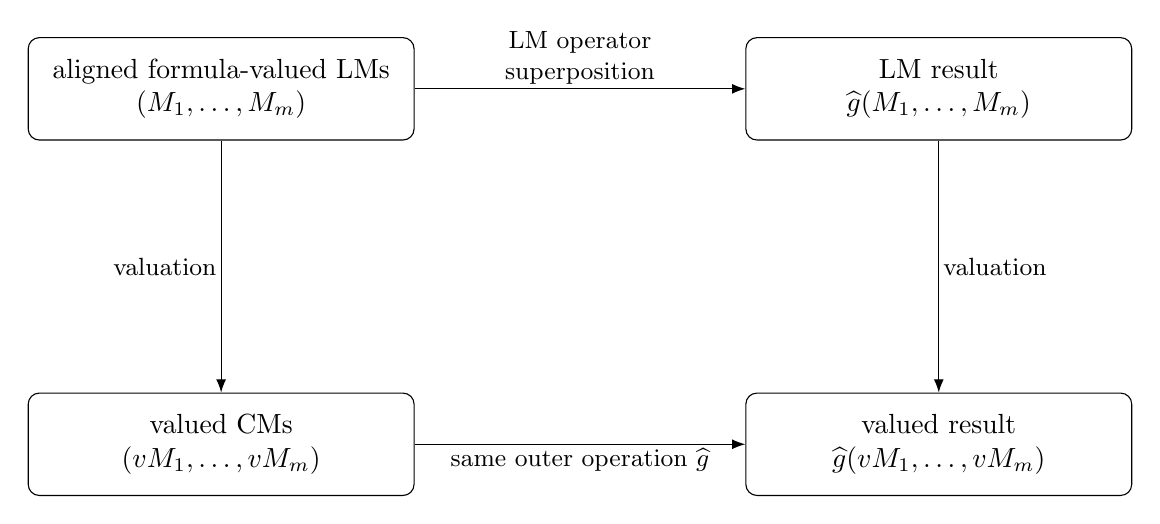
\begin{tikzpicture}[>=Latex,
  box/.style={draw,rounded corners,align=center,minimum width=49mm,minimum height=13mm,inner sep=7pt},
  lab/.style={fill=white,inner sep=1.5pt,align=center,font=\small}]
\node (mvec) [box] {aligned formula-valued LMs\\$(M_1,\ldots,M_m)$};
\node (mout) [box,right=42mm of mvec] {LM result\\$\widehat g(M_1,\ldots,M_m)$};
\node (vvec) [box,below=32mm of mvec] {valued CMs\\$(vM_1,\ldots,vM_m)$};
\node (vout) [box,below=32mm of mout] {valued result\\$\widehat g(vM_1,\ldots,vM_m)$};
\draw[->] (mvec) -- node[lab,above]{LM operator\\superposition} (mout);
\draw[->] (mvec) -- node[lab,left]{valuation} (vvec);
\draw[->] (mout) -- node[lab,right]{valuation} (vout);
\draw[->] (vvec) -- node[lab,below]{same outer operation $\widehat g$} (vout);
\end{tikzpicture}
\caption{LM-centered coherence under valuation.  The same outer Boolean operation may be applied to aligned formula-valued operators before valuation or to their valued CMs afterward.  Logical pairing and common input-frame pullbacks satisfy analogous squares because they are Boolean homomorphisms on the pointwise operator algebra.}
\label{fig:coherencesquare}
\end{figure}

\begin{remark}[Pairing preserves the running calculation]
The final line of Example~5.3 is an instance of Theorem~\ref{thm:coherence}: after the reversed implication has been transported to the common frame, pairing may be applied before or after the pointwise XOR.  The agreement-bit result $(A\Leftrightarrow X)\xor(Y\Leftrightarrow B)$ is therefore the relational image of the same aligned operator computation, not a separate identity chosen for the example.
\end{remark}

\subsection{Higher-arity logical pairing}
For formula tuples $\mathbf A=(A_1,\ldots,A_n)$ define
\begin{equation}
 \cP_f(\mathbf A;\mathbf X)
 =\bigxor_{\alpha\in\B^n}
 \cM_f(\mathbf X)[\alpha]
 \land\bigwedge_{i=1}^n A_i^{\langle\alpha_i\rangle}.
 \label{eq:npairingdef}
\end{equation}

\begin{theorem}[Higher-arity pairing and reconstruction]
For every $f:\B^n\to\B$,
\begin{equation}
 \cP_f(\mathbf A;\mathbf X)
 \equiv
 \widetilde f(A_1\Leftrightarrow X_1,\ldots,A_n\Leftrightarrow X_n).
 \label{eq:npairing}
\end{equation}
Valuation commutes with this contraction.  Moreover, for each assignment $\beta\in\B^n$,
\begin{equation}
 \cP_f\bigl((X_1^{\langle\beta_1\rangle},\ldots,X_n^{\langle\beta_n\rangle});\mathbf X\bigr)
 \equiv f(\beta),
 \label{eq:nreconstruction}
\end{equation}
so the complete labelled basis-pairing table reconstructs the truth tensor.
\end{theorem}
\begin{proof}
The weights $w_\alpha:=\bigwedge_i A_i^{\langle\alpha_i\rangle}$ form a Boolean partition of unity indexed by $\alpha$.  To make the selected index explicit, fix an arbitrary valuation $v$.  Exactly one weight is true, namely the one with $\alpha_i=v(A_i)$ for every $i$.  At that cell,
\[
 v\!\left(\cM_f(\mathbf X)[\alpha]\right)
 =f\bigl(v(A_1)\xor v(X_1)\xor1,\ldots,
         v(A_n)\xor v(X_n)\xor1\bigr),
\]
which is $f$ evaluated on the $n$ agreement bits $v(A_i\Leftrightarrow X_i)$.  Since this holds under every valuation, the selected formula is
$\widetilde f(A_1\Leftrightarrow X_1,\ldots,A_n\Leftrightarrow X_n)$, proving Equation~\eqref{eq:npairing}.  Valuation preservation follows from the same selector homomorphism.  Setting $A_i=X_i^{\langle\beta_i\rangle}$ makes the $i$th agreement bit the constant $\beta_i$, proving Equation~\eqref{eq:nreconstruction}.
\end{proof}

\begin{figure}[ht]
\centering
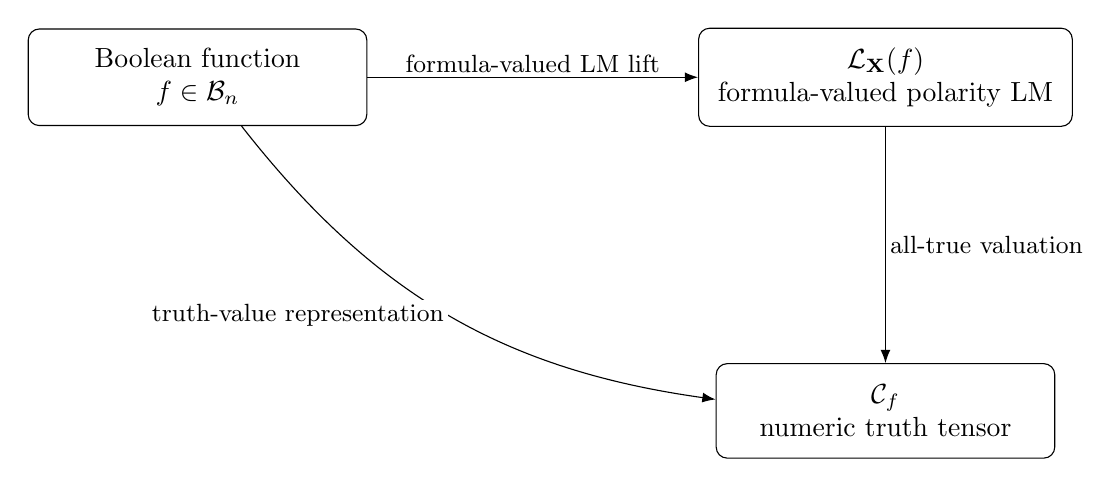
\begin{tikzpicture}[>=Latex,
  box/.style={draw,rounded corners,align=center,minimum width=43mm,minimum height=12mm,inner sep=7pt},
  lab/.style={fill=white,inner sep=1.5pt,align=center,font=\small}]
\node (f) [box] {Boolean function\\$f\in\mathcal B_n$};
\node (lm) [box,right=42mm of f] {$\mathcal L_{\mathbf X}(f)$\\formula-valued polarity LM};
\node (cm) [box,below=30mm of lm] {$\cC_f$\\numeric truth tensor};
\draw[->] (f) -- node[lab,above]{formula-valued LM lift} (lm);
\draw[->] (lm) -- node[lab,right]{all-true valuation} (cm);
\draw[->,bend right=22] (f) to node[lab,left]{truth-value representation} (cm);
\end{tikzpicture}
\caption{The LM embedding is faithful because all-true valuation recovers the numeric correspondence tensor.  Boolean superposition may be performed before or after the lift.}
\label{fig:embedding}
\end{figure}

\section{Matrix flattenings and higher-dimensional CMs}
\label{sec:flatten}

A tensor becomes a matrix after the variables are split into a row block and a column block.  This is the clean higher-dimensional generalization of the binary CM, and it also answers a terminology question: a matrix need not be square to act as a typed map.

Let $R=(i_1,\ldots,i_p)$ and $C=(j_1,\ldots,j_q)$ be an ordered partition of $\{1,\ldots,n\}$, with $p+q=n$.  For row bits $r\in\B^p$ and column bits $c\in\B^q$, let
\[
 \operatorname{assemble}_{R\mid C}(r,c)\in\B^n
\]
be the unique complete assignment whose coordinates $i_a$ equal $r_a$ and whose coordinates $j_b$ equal $c_b$.  This explicit assembly map avoids any ambiguity when the two blocks are noncontiguous or use a nonstandard order.  Empty blocks are allowed: $\B^0$ is the singleton containing the empty assignment and an empty Kronecker product is the scalar state $1$.  Thus the limiting shapes $1\times2^n$ and $2^n\times1$ are covered without a separate convention.

\begin{definition}[Correspondence-map flattening]
The $(R\mid C)$ flattening is the $2^p\times2^q$ array
\begin{equation}
 [f]_{R\mid C}[r,c]
 :=f\!\left(\operatorname{assemble}_{R\mid C}(r,c)\right).
 \label{eq:flattening}
\end{equation}
Its formula-valued counterpart $[M_f(\mathbf X)]_{R\mid C}$ is defined by the same ordered assembly of the logical tensor.  Computationally this is an axis permutation followed by a reshape of $\cC_f$.
\end{definition}

\begin{example}[A noncontiguous ordered flattening]
Let $n=3$, take $R=(3,1)$ and $C=(2)$, and set
$f(x_1,x_2,x_3)=x_1\xor(x_2\land x_3)$.  If the row bits are $r=(r_1,r_2)$ and the column bit is $c$, then
\[
 \operatorname{assemble}_{(3,1)\mid(2)}(r,c)=(r_2,c,r_1).
\]
In true-first row order $(11,10,01,00)$ and column order $(1,0)$ this gives
\[
 [f]_{(3,1)\mid(2)}=
 \begin{bmatrix}
 0&1\\
 1&0\\
 1&1\\
 0&0
 \end{bmatrix}.
\]
The example shows why the ordered assembly map is part of the type: a noncontiguous flattening is a precise reindexing, not an appeal to a visually guessed reshape.
\end{example}

The notation $[\Theta]$ remains reserved as the binary shorthand.  For higher arity, the subscript $R\mid C$ is preferable to a bare size such as $[\Theta]_4$: two different constructions can both be $4\times4$ while having different types.  In particular, a four-variable $2\mid2$ correspondence map is not the same object as the $4\times4$ coefficient-permutation matrix introduced later to rotate the four cells of a binary CM.

Under XOR--AND multiplication, $[f]_{R\mid C}$ is a linear map
\[
 \F_2^{\,2^q}\longrightarrow\F_2^{\,2^p}.
\]
It is an endomorphism only when $p=q$.  We use ``operator'' in the broad typed sense of an acting map; when strict endomorphism terminology matters, we say \emph{correspondence map} for a rectangular flattening.

Let
\[
 |x_R\rangle=\bigotimes_{k=1}^p|x_{i_k}\rangle,
 \qquad
 |x_C\rangle=\bigotimes_{\ell=1}^q|x_{j_\ell}\rangle.
\]
These Kronecker products are one-hot states of lengths $2^p$ and $2^q$.
\begin{theorem}[Rectangular bra--map--ket selection]
For every bipartition $R\mid C$,
\begin{equation}
 \langle x_R|[f]_{R\mid C}|x_C\rangle
 =f(x_1,\ldots,x_n).
 \label{eq:matrixselection}
\end{equation}
Thus square shape is not required for a scalar bra--matrix--ket contraction; the left and right state spaces simply have different dimensions when $p\ne q$.
\end{theorem}
\begin{proof}
The grouped row and column states are one-hot and select the single matrix entry indexed by the complete assignment.
\end{proof}

\begin{remark}[Comparison with quantum terminology]
In ordinary linear algebra, a rectangular matrix is a linear map between different vector spaces, whereas a square matrix is an endomorphism.  Quantum observables and POVM effects on one Hilbert space are square; more general quantum processes can involve maps between input and output spaces of different dimensions.  A tensor reshaping does not automatically preserve a physical-observable interpretation.  The present Boolean construction requires only the typed linear-map statement in \eqref{eq:matrixselection}, not a quantum measurement analogy.
\end{remark}

\begin{remark}[Exact size boundary]
The tensor, a length-$2^n$ truth vector, and every $2^p\times2^q$ flattening contain the same $2^n$ Boolean entries.  Reshaping may change computational locality, cache behavior, or available algorithms, but it does not compress an arbitrary truth relation.  Any benchmark advantage of rectangular rather than square flattenings is therefore an implementation result rather than a smaller information content.
\end{remark}

\begin{figure}[ht]
\centering
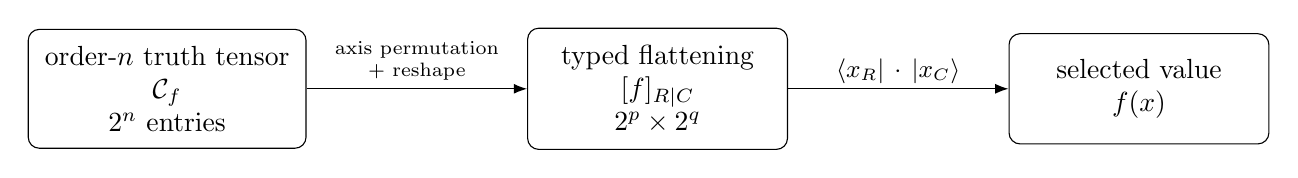
\begin{tikzpicture}[>=Latex,
  box/.style={draw,rounded corners,align=center,minimum width=33mm,minimum height=14mm,inner sep=6pt},
  lab/.style={fill=white,inner sep=1.5pt,align=center,font=\small}]
\node (tensor) [box] {order-$n$ truth tensor\\$\cC_f$\\$2^n$ entries};
\node (map) [box,right=28mm of tensor] {typed flattening\\$[f]_{R\mid C}$\\$2^p\times2^q$};
\node (scalar) [box,right=28mm of map] {selected value\\$f(x)$};
\draw[->] (tensor) -- node[fill=white,inner sep=1pt,align=center,font=\scriptsize,above=2pt]{axis permutation\\+ reshape} (map);
\draw[->] (map) -- node[lab,above]{$\langle x_R|\,\cdot\,|x_C\rangle$} (scalar);
\end{tikzpicture}
\caption{Higher-dimensional CMs are typed matrix flattenings of the same $2^n$-entry correspondence tensor.  Rectangular maps remain valid operands in a bra--map--ket contraction.}
\label{fig:flattening}
\end{figure}

\section{Building higher-dimensional operators from lower-dimensional ones}
\label{sec:blocklift}

Let $g:\B^p\to\B$ and $h:\B^q\to\B$ act on disjoint variable blocks, and let $\Theta$ be a binary outer connective.  If $t_g,t_h$ are the true-first truth vectors, define
\begin{equation}
 \cO_\Theta(t_g,t_h)[a,b]:=t_g[a]\,\Theta\,t_h[b].
 \label{eq:outerlift}
\end{equation}
For formula variables on the two blocks, let $\mathbf X_A^{\langle a\rangle}$ denote componentwise polarity substitution, so its $i$th component is $X_i^{\langle a_i\rangle}$.  Define the polarity vectors
\begin{equation}
 \ell_g(\mathbf X_A)[a]:=\widetilde g(\mathbf X_A^{\langle a\rangle}),\qquad
 \ell_h(\mathbf X_B)[b]:=\widetilde h(\mathbf X_B^{\langle b\rangle}).
 \label{eq:polarityvectors}
\end{equation}

\begin{theorem}[Block-lift theorem]
If
\[
 f(a,b)=g(a)\,\Theta\,h(b),
\]
then
\begin{align}
 [f]_{A\mid B}&=\cO_\Theta(t_g,t_h),
 \label{eq:blocklift}\\
 [M_f(\mathbf X)]_{A\mid B}&=\cO_{\widetilde\Theta}\bigl(\ell_g(\mathbf X_A),\ell_h(\mathbf X_B)\bigr).
 \label{eq:symbolicblocklift}
\end{align}
Valuation commutes with both constructions.
\end{theorem}
\begin{proof}
At the entry indexed by $(a,b)$, the numeric right side is $g(a)\Theta h(b)=f(a,b)$.  The formula-valued statement is the same identity after polarity substitution, and valuation preserves $\Theta$.
\end{proof}

\begin{theorem}[Rank and conjunctive/XOR separability]
For a fixed bipartition $A\mid B$:
\begin{enumerate}
\item $f(a,b)=g(a)\land h(b)$ for some Boolean functions $g,h$ if and only if
\[
 \operatorname{rank}_{\F_2}[f]_{A\mid B}\le 1.
\]
For a nonzero function the factorization is the ordinary rank-one factorization
\begin{equation}
 [f]_{A\mid B}=t_g\,t_h^T,
 \label{eq:separable}
\end{equation}
and over $\F_2$ the nonzero factors are unique.
\item More generally, the minimum integer $k\ge0$ for which
\begin{equation}
 f(a,b)=\bigxor_{i=1}^{k} g_i(a)\land h_i(b)
 \label{eq:xorrankdecomp}
\end{equation}
equals $\operatorname{rank}_{\F_2}[f]_{A\mid B}$.  The empty XOR for $k=0$ is defined to be $0$, so the zero function has minimum $k=0$.
\end{enumerate}
The formula-valued flattening of a rank-one term factorizes analogously as the outer product of the two polarity vectors.
\end{theorem}
\begin{proof}
A conjunctive factor $g(a)\land h(b)$ has matrix $t_g t_h^T$ and therefore rank at most one.  Conversely, every nonzero rank-one matrix over $\F_2$ is $uv^T$ for nonzero Boolean vectors $u,v$, which are the truth vectors of unique Boolean functions on the two blocks; the zero matrix is obtained by taking one factor identically zero.  For the second statement, every summand in~\eqref{eq:xorrankdecomp} has rank at most one, so $k$ is at least the matrix rank.  A rank factorization supplies exactly that many rank-one outer products, proving equality.
\end{proof}

This gives a precise modern form of the separability/factorization idea already present in the original LM manuscript \cite{Droncheff2018}.  The statement concerns ordinary $\F_2$ rank and XOR decomposition, not the different OR-based notion usually called Boolean rank.  The value also depends on the chosen bipartition: repartitioning the variables can change the flattening rank.

\begin{example}[A $4\times4$ correspondence map]
Let
\[
 g(W,X)=W\xor X,\qquad
 h(Y,Z)=\neg Y\land Z,\qquad
 f=g\Rightarrow h.
\]
In true-first order $(11,10,01,00)$,
\[
 t_g=(0,1,1,0),\qquad t_h=(0,0,1,0).
\]
The $2\mid2$ block lift gives
\begin{equation}
 [f]_{(W,X)\mid(Y,Z)}=
 \begin{bmatrix}
 1&1&1&1\\
 0&0&1&0\\
 0&0&1&0\\
 1&1&1&1
 \end{bmatrix}.
 \label{eq:fourbyfour}
\end{equation}
This recovers the useful content of the historical four-variable construction without claiming that four variables intrinsically require a unique $4\times4$ shape.
\end{example}

\section{Signed variable frames in arbitrary arity}
\label{sec:frames}

For numeric truth tensors, input permutations and polarity changes form the signed-permutation action.  Let $\sigma\in S_n$ and $\epsilon\in\B^n$, and define
\begin{equation}
 \phi_{\sigma,\epsilon}(x)_i=x_{\sigma(i)}\xor\epsilon_i.
 \label{eq:signedmap}
\end{equation}
Define the numeric pullback $T_{\sigma,\epsilon}$ by
\[
 (T_{\sigma,\epsilon}C)[x]:=C[\phi_{\sigma,\epsilon}(x)].
\]
With this convention the pullbacks form a right action: $T_{\phi}T_{\psi}=T_{\psi\circ\phi}$.  This fixes the composition direction rather than leaving it implicit.
\begin{theorem}[Signed-frame action]
For every $f:\B^n\to\B$,
\begin{equation}
 \cC_{f\circ\phi_{\sigma,\epsilon}}
 =T_{\sigma,\epsilon}\cC_f.
 \label{eq:signedaction}
\end{equation}
The transformations form the standard signed-permutation group $(C_2)^n\rtimes S_n$ on the input frame.  Output negation is a separate $C_2$ action on the coefficients.
\end{theorem}

For the symbolic level it is useful to state the transport law without leaving the mask placement implicit.  Let $P_\sigma$ permute tuples by $(P_\sigma z)_i=z_{\sigma(i)}$, and define the signed reference tuple by
\[
 \phi_{\sigma,\epsilon}(\mathbf X)_i
 :=X_{\sigma(i)}^{\langle 1\xor\epsilon_i\rangle}.
\]
Then for every $f:\B^n\to\B$ and every polarity index $\alpha\in\B^n$,
\begin{equation}
 \boxed{
 \mathcal L_{\mathbf X}(f\circ\phi_{\sigma,\epsilon})[\alpha]
 =\mathcal L_{P_\sigma\mathbf X}(f)[P_\sigma\alpha\xor\epsilon]
 =\mathcal L_{\phi_{\sigma,\epsilon}(\mathbf X)}(f)[P_\sigma\alpha].}
 \label{eq:symbolic-signed-transport}
\end{equation}
All three formulas are the same Boolean term after substitution.  Equation~\eqref{eq:symbolic-signed-transport} also prevents a common implementation error: the polarity mask $\epsilon$ may be represented in the reference tuple or in the slot index, but not independently in both.  Applying the same mask twice cancels it.  In arity one with $f(x)=x$, $X=1$, $\alpha=1$, and $\epsilon=1$, the desired transported value is $0$; a double flip incorrectly returns $1$.

Under a matrix flattening, the same action appears as row/column permutations, transpositions or block transpositions, and---when a variable moves across the chosen bipartition---a reshape.  The symbolic identity above specifies the corresponding variable renaming and polarity substitution exactly.

\begin{theorem}[Frame changes commute with pointwise composition]
For any common numeric reindexing $T$ and outer Boolean operation $g$,
\begin{equation}
 T\,\widehat g(\cC_{f_1},\ldots,\cC_{f_m})
 =\widehat g(T\cC_{f_1},\ldots,T\cC_{f_m}).
 \label{eq:framecommutes}
\end{equation}
The formula-valued version holds when the same frame change includes the corresponding variable relabeling/polarity substitution.
\end{theorem}

\subsection{Relation to NPN transformations}

NPN stands for \emph{input Negation, input Permutation, output Negation}.  Two Boolean functions are NPN-equivalent when one can be obtained from the other by these transformations.  NPN classification is standard in logic synthesis, where it is useful for canonicalizing small truth functions and reusing optimized implementations \cite{Mishchenko2006,Zhou2019}.

For binary CMs the transformations are visually explicit:
\begin{center}
\begin{tabular}{ll}
input permutation & $[\Theta]\mapsto[\Theta]^T$,\\
negate left input & $[\Theta]\mapsto[\Updownarrow][\Theta]$,\\
negate right input & $[\Theta]\mapsto[\Theta][\Updownarrow]$,\\
negate output & $[\Theta]\mapsto J\xor[\Theta]$ entrywise.
\end{tabular}
\end{center}
Thus the CM frame calculus realizes the binary NPN moves as simple matrix transformations.  This is useful for frame normalization and comparison, but the existence of NPN equivalence itself is not a novelty claim.

\section{Relationship to ANF and other coordinate representations}
\label{sec:anf}

The CM/LM architecture should not be confused with an algebraic-normal-form coefficient vector.  A correspondence tensor stores truth values; ANF stores coefficients of square-free monomials.  The two are related by Boolean M\"obius inversion.

Write
\begin{equation}
 f(x_1,\ldots,x_n)
 =\bigxor_{S\subseteq[n]}
 a_S\bigwedge_{i\in S}x_i.
 \label{eq:anf}
\end{equation}
If $t_T=f(1_T)$ denotes the truth value on the assignment whose support is $T$, then
\begin{equation}
 t_T=\bigxor_{S\subseteq T}a_S,
 \qquad
 a_S=\bigxor_{T\subseteq S}t_T.
 \label{eq:mobius}
\end{equation}

\begin{proposition}[Top ANF coefficient as correspondence parity]
For every Boolean function of positive arity $n\ge1$,
\begin{equation}
 a_{[n]}=\bigxor_{x\in\B^n}f(x).
 \label{eq:topparity}
\end{equation}
Hence $\deg f=n$ if and only if the correspondence tensor has odd Hamming weight.
\end{proposition}
\begin{proof}
The second relation in \eqref{eq:mobius}, applied to $S=[n]$, XORs every truth value.  The coefficient $a_{[n]}$ is one exactly when the full monomial is present.
\end{proof}

\begin{corollary}[Binary nonlinearity parity criterion]
For the binary correspondence matrix
\[
 [f]_{X\mid Y}=\begin{bmatrix}f_{11}&f_{10}\\f_{01}&f_{00}\end{bmatrix},
\]
the coefficient of $XY$ is
\[
 a_{XY}=f_{11}\xor f_{10}\xor f_{01}\xor f_{00}.
\]
Thus a two-variable Boolean function has algebraic degree exactly $2$ if and only if its CM has odd Hamming weight.
\end{corollary}

This parity result belongs naturally in a CM/LM foundations paper because it relates an immediately visible operator invariant to ordinary Boolean degree.  A stronger statement available in the separate cyclic-lift program says that, after the four truth coefficients are embedded into a particular rotation-generated algebra, the same parity becomes the unit criterion.  That conclusion depends on the additional algebra and is not used here.

For two variables, one may also compare with an STP logical structure matrix.  Under the common delta encoding $1\mapsto(1,0)^T$, $0\mapsto(0,1)^T$ and column order $(11,10,01,00)$, if
\[
 t=\vecop([f]_{X\mid Y})^T=(f_{11},f_{10},f_{01},f_{00}),
\]
then one binary-output structure matrix is
\[
 M_f^{\mathrm{STP}}=\begin{bmatrix}t\\\neg t\end{bmatrix}.
\]
This is an external representation of the same truth function, not a component of the formula-valued LM.  Likewise ANF coefficients are reached by \eqref{eq:mobius}, not by positive valuation.

\section{A boundary around literal CM rotation}
\label{sec:rotationboundary}

Literal quarter-turn rotation of a displayed $2\times2$ CM is already part of the signed frame geometry.  It should be distinguished from the later step of imposing a cyclic multiplication on the four coefficient positions.

Define clockwise rotation by
\begin{equation}
 \rot\begin{bmatrix}a&b\\c&d\end{bmatrix}
 =\begin{bmatrix}c&a\\d&b\end{bmatrix}.
 \label{eq:rotation}
\end{equation}
If $[\Theta']:=\rot([\Theta])$, then the associated truth functions satisfy
\begin{equation}
 f_{\Theta'}(x,y)=f_\Theta(\neg y,x).
 \label{eq:rotationlogic}
\end{equation}
Thus $\rot^4=I$ and the quarter turn is a signed coordinate transformation.

To make the coefficient action explicit, use true-first row-major vectorization
\[
 \vecop([\Theta])=(\Theta_{11},\Theta_{10},\Theta_{01},\Theta_{00})^T.
\]
Then the $4\times4$ permutation matrix
\begin{equation}
 \mathcal R_{\circlearrowright}:=
 \begin{bmatrix}
 0&0&1&0\\
 1&0&0&0\\
 0&0&0&1\\
 0&1&0&0
 \end{bmatrix}
 \label{eq:rhoquarter}
\end{equation}
satisfies
\[
 \mathcal R_{\circlearrowright}\vecop([\Theta])
 =\vecop(\rot([\Theta])).
\]
For XNOR,
\[
 \vecop([\Leftrightarrow])=
 \begin{bmatrix}1\\0\\0\\1\end{bmatrix},
\]
so
\[
 \mathcal R_{\circlearrowright}
 \begin{bmatrix}1\\0\\0\\1\end{bmatrix}
 =
 \begin{bmatrix}0\\1\\1\\0\end{bmatrix}
 =\vecop([\Updownarrow]).
\]
This is the worked meaning of
\[
 \mathcal R_{\circlearrowright}\vecop([\Leftrightarrow])
 =\vecop([\Updownarrow]).
\]
The symbol $\mathcal R_{\circlearrowright}$ is intentionally not written as $[\Theta]_4$: it is an operator acting on the four coefficients of a \emph{binary} CM, whereas a $4\times4$ four-variable correspondence map such as $[f]_{(W,X)\mid(Y,Z)}$ acts between grouped logical state spaces.  Equal matrix size does not imply equal type.

The historical Impax observation also sits naturally here.  Since $[\Leftrightarrow]$ and $[\Updownarrow]$ have complementary supports,
\[
 [\Leftrightarrow]\xor[\Updownarrow]=J,
\]
the all-ones tautological CM.  The old overlay glyph may be retained as historical notation, while $J$ or $[\top]$ is algebraically unambiguous.

A separate phase construction begins only after an additional multiplication is imposed on the four cyclic coefficient positions.  Identifying those positions with $1,g,g^2,g^3$ and adding cyclic convolution yields
\[
 \F_2[C_4]\cong\F_2[g]/(g^4-1)
 \cong\F_2[u]/(u^4),\qquad u=1+g.
\]
That convolution is not the original $2\times2$ CM matrix product, not pointwise conjunction, and not LM pairing.  Its algebraic consequences therefore lie outside the present calculus.  The only fact needed here is the logical origin of the quarter-turn action as a signed coordinate transformation.


\section{Computational interpretation without a performance claim}
\label{sec:computational}

The operator calculus has an immediate compiler interpretation.  If two subexpressions depend on the same variables but use different operand order or polarity, the signed-frame action can normalize both to one declared frame.  Section~\ref{sec:operatoronoperator} then permits the outer connective to be evaluated pointwise on their operators.  This can collapse repeated Boolean work before later expansion or evaluation.

The companion computational manuscript \cite{TheoryCompiler2026} develops this idea as a typed pair compiler with pure-structural, hybrid-retabulation, whole-retabulation, and fallback paths.  The mathematical content needed here is only the invariant: fusion is sound when the operands refer to the same assignments in the same declared frame.

This structural simplification should not be confused with a claim of unique or universal speedup.  Packed truth-function optimizers and logic-synthesis methods can perform closely related local reductions, and the raw same-frame pointwise law itself has prior art.  The computational question is therefore empirical: whether explicit typed frame recognition and fusion provide a useful implementation boundary on relevant workloads.  Timing, memory, comparator design, and any positive or negative performance evidence belong to the companion computational paper and are not used as evidence for the foundations claims here.

\section{Relationship to prior operator formalisms and claim boundary}
\label{sec:related}

The CM/LM calculus sits among several established representations.  Table~\ref{tab:related} is a type map rather than a novelty verdict.

\begin{table}[ht]
\centering\footnotesize
\begin{tabular}{L{.15\linewidth}L{.20\linewidth}L{.22\linewidth}L{.31\linewidth}}
\toprule
Family & Primary object & Typical operation & Relation here\\
\midrule
Boolean matrices & Binary matrices & Boolean products and transformations & Broad Boolean-matrix antecedent \cite{Edwards1972}.\\
Matrix/vector logic & Truth vectors and matrix gates & Linear or multilinear operator action & Strong antecedent for connective-as-operator viewpoints \cite{Stern1988,Mizraji1992,Mizraji2008}.\\
Bricken matrix-logic notes & $2\times2$ Boolean relation matrices and two-component truth vectors & Explicit $\langle x|B|y\rangle$ evaluation, Boolean matrix algebra, complements, transforms, and operations on logical matrices & Internally dated March 1997; direct antecedent for logical bra--matrix--ket notation and binary operator matrices.  Public-release chronology remains to be verified \cite{Bricken1997}.\\
STP logic & $2\times2^n$ logical structure matrices & Semi-tensor products and logical structure operations & External numeric representation, not the same type as a formula-valued LM \cite{ChengQi2010,ZhaoSTP}.\\
Boolean matrix calculus & Boolean matrices and truth vectors over XOR/AND & Matrix calculus plus arbitrary binary outer operation on corresponding truth-vector entries & Direct antecedent for the raw same-frame numerical superposition law; Prop.~3.3 states $m_{f\Phi g}=m_f\Phi m_g$ \cite{Cheng2011}.\\
NPN/LUT synthesis & Packed truth functions and shared DAGs & Input/output phase, input permutation, cut matching & Strong operational antecedent for frame transformations and small-function reuse \cite{Mishchenko2006,Zhou2019}.\\
ANF & Square-free polynomial coefficients & M\"obius transform and polynomial arithmetic & Different coordinates, related by Boolean M\"obius inversion.\\
Eigenlogic & Commuting projectors on interpretation space & Truth values as eigenvalues and logical interpretations as eigenvectors & Direct prior art for spectral logical observables; raw $2\times2$ CMs have a different $\F_2$ spectrum, while $\mathsf D_\Theta$ gives the diagonal truth-observable bridge \cite{Toffano2020,DuboisToffano2016}.\\
CM/LM calculus & Typed truth tensor plus polarity-equivariant formula tensor & Valuation, pairing, frame transport, aligned pointwise superposition, matched-frame kernel product, and block lift & Integrated object studied in this paper.\\
\bottomrule
\end{tabular}
\caption{Representation and operation types.  Individual matrix, truth-table, frame, and pointwise operations have substantial prior art; the paper studies their particular integration in the CM/LM architecture.}
\label{tab:related}
\end{table}

A recent neighboring construction is the Binary Matrix Product (BMP) representation of Boolean functions \cite{Usturali2025}.  BMPs use products of binary matrices as compressed normal forms closely related to BDDs, with an explicit computational aim.  The correspondence tensor and its flattenings here instead retain all $2^n$ truth coefficients and make no compression claim.  The comparison is useful precisely because both use matrix language for Boolean functions while solving different representation problems.

\subsection{Boolean closure as a claim boundary}
\begin{proposition}[Core Boolean closure]
Starting from a formula-valued LM or logical tensor, polarity substitution, logical-state construction, XOR--AND contraction, pointwise Boolean superposition, block outer composition, support difference, and signed-frame reindexing remain internal to Boolean algebra.  After valuation, the corresponding numeric operations remain in $\F_2$.
\end{proposition}
\begin{proof}
Each symbolic construction is formed from Boolean term operations, substitution, finite indexing, or reindexing.  Boolean valuation preserves the term operations and yields only $0$ or $1$ coefficients.  No step requires an extension of the scalar domain.
\end{proof}
No real, complex, negative, or otherwise non-Boolean scalar is needed for the core calculus.  This closure is not by itself a historical priority claim.  Its value is to state exactly which transformations belong to the CM/LM system before any optional extension---for example the cyclic phase multiplication---is added.

The central mathematical contribution of the paper is architectural and structural rather than a claim that any one elementary operation is new.  Numeric correspondence tensors and formula-valued LMs provide two typed realizations of the same Boolean functions; aligned operators can themselves be operands of arbitrary Boolean superposition; and Theorem~\ref{thm:coherence} shows that valuation, common frame transport, and logical pairing all respect that superposition.  Higher-dimensional block construction and Boolean closure complete the calculus.  The orbit-lift and polarity-equivariance theorems identify the symbolic object cleanly, but their underlying group-action mechanism is treated as standard.

\section{Discussion}

\subsection{What makes this a calculus rather than a list of identities}

The formula-valued LM is the organizing symbolic object of the calculus.  Boolean superposition acts directly on aligned LMs; valuation sends the result to numeric correspondence tensors; signed input-frame changes reindex the symbolic and numeric levels consistently; and logical pairing is itself a Boolean homomorphism for the same pointwise operation.  The raw cellwise truth-vector law is classical, but the LM layer records which formulas and polarities each cell means, so the frame condition becomes an explicit semantic type rather than an implicit ordering convention.  Theorem~\ref{thm:coherence} collects these compatibility laws.

Two structural results explain why the pieces fit.  The frame normal form $[M_{X\Theta Y}]=\mathsf S_X[\Theta]\mathsf S_Y$ identifies the symbolic polarity matrix as an invertible change of Boolean frame, while the partition-selector theorem explains why pairing preserves arbitrary outer Boolean operations.  Ordinary matrix multiplication then has its own matched-intermediate-frame law, separate from pointwise superposition.  Together these distinguish a typed calculus from a mere list of matrix-decorated truth identities without claiming a new underlying Boolean algebra.

Higher-dimensional matrices then arise from variable grouping rather than from a new truth domain.  The order-$n$ tensor is primary; a $2^p\times2^q$ matrix is one flattening.  This removes ambiguity from historical higher-dimensional descriptions and makes recursive block structure explicit.

\subsection{Scope beyond the present calculus}

Literal CM rotation is included because it is already a signed-frame action.  A cyclic convolution on the four coefficient positions would introduce a second multiplication and a different algebraic object; none of the results in this paper depends on that extension.  Questions about such a phase algebra, modal interpretations, or operator-valued enrichments are therefore deferred rather than used to enlarge the claims of the present calculus.

\subsection{Open structural questions}

Three directions are especially natural.
\begin{enumerate}
  \item \textbf{Abstract formulation.}  The faithful preservation of Boolean superposition suggests a clone-theoretic or equivariant description of the LM lift and its frame action.
  \item \textbf{Canonicalization.}  Signed permutations and NPN equivalence provide natural orbit relations; their interaction with formula-level equivalence and efficient canonical forms deserves separate study.
  \item \textbf{Empirical utility.}  The typed frame contract is exact, but whether it improves a compiler or symbolic workflow is an empirical question to be tested in the computational companion rather than assumed here.
\end{enumerate}

\section{Conclusion}

The binary notation $\Theta$ versus $[\Theta]$ distinguishes a logical operator from its compact numeric representation, while the formula-valued LM $[M_{X\Theta Y}]$ supplies the symbolic polarity layer that organizes the present calculus.  Its valuation recovers $[\Theta]$ in the appropriate signed operand frame, and its logical pairing returns an exact relationship formula.

The central structural statement is therefore LM-centered coherence.  Aligned formula-valued logical operators may themselves be combined as first-class operands of arbitrary Boolean outer operations; valuation transports that computation to numeric CMs, logical pairing preserves it relationally, and signed input-frame actions preserve its typing.  The frame normal form and selector characterization explain this coherence structurally; the orbit/equivariance results classify the LM image; Boolean closure states the scalar boundary.  The CM-level pointwise law remains important computationally, but it is treated as the valued numeric image of the broader symbolic construction rather than as the principal novelty claim.

An $n$-variable correspondence tensor may be flattened into a $2^p\times2^q$ correspondence map for any declared bipartition.  Rectangular maps remain genuine typed linear maps from $\F_2^{2^q}$ to $\F_2^{2^p}$ and still participate in bra--map--ket selection.  Block lifts and the rank/separability theorem recover useful higher-dimensional structure from lower-dimensional subfunctions without changing the $2^n$ information bound: the flattening rank is exactly the minimum number of conjunctive factors in an XOR decomposition across the declared bipartition.

The paper also clarifies several boundaries.  OR--AND and XOR--AND agree on one-hot selection but differ for general linear combinations; XOR is retained to preserve the $\F_2$ coefficient algebra.  NPN transformations are standard and are realized here as explicit frame operations rather than claimed as new.  ANF is a different coordinate system.  Ordinary $\F_2$ eigenanalysis supplies algebraic signatures of square CMs, but those eigenvalues are not the truth values of the connective; an Eigenlogic-style diagonal truth observable lives instead on the four-dimensional interpretation space.  Finally, the $4\times4$ quarter-turn permutation $\mathcal R_{\circlearrowright}$ acts on the four coefficients of a binary CM and must not be confused with a $4\times4$ four-variable correspondence map.  Adding cyclic convolution to that coefficient rotation produces the separate phase algebra rather than another axiom of the CM/LM foundations.

\appendix

\section{Spectral boundary and representative compact-CM examples}
\label{sec:spectrum}

Because a binary CM is a square matrix over $\F_2$, ordinary finite-field eigenanalysis is available.  It should, however, be distinguished both from the older eigenproblem for matrices over a Boolean algebra and from the quantum-mechanical notion of an observable.  Boolean-matrix eigenproblems have been studied since at least Rutherford and Blyth \cite{Rutherford1965,Blyth1967}; those works use Boolean-algebra matrix operations rather than necessarily the XOR--AND field algebra fixed here.

For $A\in M_2(\F_2)$, define the characteristic polynomial in the ordinary field sense,
\[
 \chi_A(\lambda)=\det(\lambda I-A)
 =\lambda^2+\operatorname{tr}(A)\lambda+\det(A),
\]
where subtraction and addition coincide in characteristic two.  The resulting spectrum is an algebraic signature of the CM, but it is not the truth table of the connective.

\begin{table}[ht]
\centering
\small
\begin{tabular}{L{0.14\textwidth}L{0.18\textwidth}L{0.22\textwidth}L{0.34\textwidth}}
\toprule
CM & characteristic polynomial over $\F_2$ & $\F_2$ eigenstructure & interpretation of the example \\
\midrule
$[\land]=\left[\begin{smallmatrix}1&0\\0&0\end{smallmatrix}\right]$
& $\lambda(\lambda+1)$
& $|1\rangle$ has eigenvalue $1$; $|0\rangle$ has eigenvalue $0$
& idempotent projection in the $\F_2$ linear-algebra sense.\\
$[\Leftrightarrow]=I$
& $(\lambda+1)^2$
& every nonzero vector has eigenvalue $1$
& identity operator.\\
$[\Updownarrow]=\left[\begin{smallmatrix}0&1\\1&0\end{smallmatrix}\right]$
& $(\lambda+1)^2$
& only the line spanned by $(1,1)^T$ is an eigenspace
& involutory but not diagonalizable over $\F_2$; the true/false basis states are exchanged rather than observed as eigenstates.\\
$[\lor]=\left[\begin{smallmatrix}1&1\\1&0\end{smallmatrix}\right]$
& $\lambda^2+\lambda+1$
& no eigenvalue in $\F_2$; roots lie in $\F_4$
& a valid logical connective despite having no $\F_2$ eigenvector.\\
\bottomrule
\end{tabular}
\caption{Representative $\F_2$ spectra of binary CMs.  The examples show why the raw CM spectrum is useful algebraically but cannot by itself serve as the truth-value spectrum of a logical observable.}
\label{tab:cmspectrum}
\end{table}

Table~\ref{tab:cmspectrum} gives a decisive boundary.  If raw CM eigenvalues were to be interpreted directly as logical measurement outcomes, OR would already be problematic: it has no eigenvalue in $\F_2$, while XOR has only the repeated eigenvalue $1$.  The four truth values of a binary connective are therefore not, in general, the eigenvalues of its $2\times2$ CM.

There is nevertheless a small projector-like subclass.  Under the declared XOR--AND matrix product, exactly eight of the sixteen binary CMs satisfy $A^2=A$.  Exactly four are also symmetric: the four diagonal CMs
\[
 [0],\qquad [\neg\lor],\qquad [\land],\qquad [\Leftrightarrow].
\]
These are algebraic projection matrices over $\F_2$ (and the same $0$--$1$ arrays are orthogonal projectors over ordinary real scalars when viewed in the standard basis).  The fact that only a proper subset of the sixteen compact CMs has this form is another reason not to identify the raw CM family wholesale with quantum observables.  This finite classification is an elementary structural observation rather than a novelty claim.
Indeed, for $A=\left[\begin{smallmatrix}a&b\\c&d\end{smallmatrix}\right]$, the equation $A^2=A$ is equivalent over $\F_2$ to $bc=0$ together with $b(a\xor d\xor1)=c(a\xor d\xor1)=0$, which has eight binary solutions.  Adding $A^T=A$ forces $b=c=0$, leaving the four diagonal matrices above.

\subsection{Matrix-element semantics versus spectral truth values}
The native CM/LM semantics has already been established in Proposition~\ref{prop:cmselection} and Corollary~\ref{cor:basisreconstruction}: truth coefficients are recovered as labelled bra--operator--ket matrix elements, and arbitrary logical pairing returns a Boolean relationship formula.  This is relational matrix-element semantics, not spectral measurement; it supplies neither Born probabilities nor state collapse.  Bricken's technical note provides direct prior art for the numeric bra--matrix--ket viewpoint \cite{Bricken1997}.  The formula-valued LM, its frame normal form, and the agreement-bit pairing architecture are the additional structures studied here.

Eigenlogic takes a different route.  On the four-dimensional interpretation space with canonical assignment basis $|11\rangle,|10\rangle,|01\rangle,|00\rangle$, a binary connective $\Theta$ canonically determines the diagonal operator
\begin{equation}
 \mathsf D_\Theta
 :=\operatorname{diag}(\Theta_{11},\Theta_{10},\Theta_{01},\Theta_{00}).
 \label{eq:diagobservable}
\end{equation}
This $4\times4$ operator is a projector over ordinary real or complex scalars because its diagonal entries are $0$ or $1$; its eigenvectors are the four interpretation basis states and its eigenvalues are exactly the truth-table outputs.  That is the spectral logic used by Eigenlogic in a more general operator setting \cite{Toffano2020,DuboisToffano2016}.  Equation~\eqref{eq:diagobservable} therefore gives a useful \emph{spectral truth-observable representation} associated with a CM if a spectral interpretation is desired, but $\mathsf D_\Theta$ is a different representation from the compact $2\times2$ CM $[\Theta]$.  In the native CM representation, truth is read through the labelled matrix elements of Proposition~\ref{prop:cmselection} and Corollary~\ref{cor:basisreconstruction}, not through the spectrum.

Formula-valued LMs also admit algebraic eigenvalue questions, since their entries lie in a commutative Boolean ring.  Ring-valued spectra are less rigid than field spectra, so the safest intrinsic object at present is the \emph{valuation spectral profile}
\begin{equation}
 \Sigma_M:v\longmapsto\operatorname{Spec}_{\F_2}(v(M)).
 \label{eq:valspectralprofile}
\end{equation}
For $M=[M_{X\Theta Y}]$, valuation produces row and column reversals of $[\Theta]$.  Independent left and right reversals need not be similarity transformations, so the $\F_2$ spectrum can vary with the valuation; simultaneous conjugate reversals preserve it.  Whether this profile supplies a useful invariant of formula-valued LMs is an open algebraic question.  Nothing in this paper interprets it as a physical observable without additional state, effect, and probability postulates.




\section{Binary LM basis expansion}
\label{app:basis}

Let $b_1=1$, $b_2=0$, $X_1=X$, $X_2=\neg X$, $Y_1=Y$, $Y_2=\neg Y$, and $c_{ij}=b_i\Theta b_j$.  Define the formula-valued outer product
\[
 |X_i\rangle\langle Y_j|
 =\begin{bmatrix}
 X_i\land Y_j&X_i\land\neg Y_j\\
 \neg X_i\land Y_j&\neg X_i\land\neg Y_j
 \end{bmatrix}.
\]
Then
\begin{equation}
 [M_{X\Theta Y}]=\bigxor_{i,j\in\{1,2\}}
 c_{ij}|X_i\rangle\langle Y_j|.
 \label{eq:lmbasis}
\end{equation}
The upper-left entry is the disjoint-minterm expansion
\[
 c_{11}XY\xor c_{12}X\neg Y\xor c_{21}\neg X Y\xor c_{22}\neg X\neg Y,
\]
which is exactly $X\Theta Y$.  Exchanging the $Y$ polarity gives the upper-right entry, exchanging the $X$ polarity gives the lower-left entry, and exchanging both gives the lower-right entry.  Thus \eqref{eq:lmbasis} is equivalent to the direct binary definition \eqref{eq:binarylm}.

\section{Compatibility identities}

The principal maps of the calculus satisfy the following compatibility relations whenever the displayed expressions are typed:
\begin{align*}
 v\bigl(\widehat g(T_1,\ldots,T_m)\bigr)
 &=\widehat g(vT_1,\ldots,vT_m),\\
 T\,\widehat g(\cC_{f_1},\ldots,\cC_{f_m})
 &=\widehat g(T\cC_{f_1},\ldots,T\cC_{f_m}),\\
 v_{\mathbf1}(\tau_\delta\mathcal L_{\mathbf X}(f))
 &=\pi_\delta\cC_f.
\end{align*}
The first says that valuation commutes with Boolean superposition; the second that a common frame reindexing commutes with pointwise composition; and the third that valuation intertwines symbolic polarity changes with numeric axis reversals.  These identities are the concise algebraic content behind the commuting diagrams used in the main text.

\section{Notation and convention table}

\begin{center}\small
\begin{tabular}{p{.25\linewidth}p{.64\linewidth}}
\toprule
Symbol & Meaning\\
\midrule
$\Theta$ & Binary logical operator variable/connective.\\
$[\Theta]$ & Numeric $2\times2$ CM representing $\Theta$ in true-first order.\\
$[M_{X\Theta Y}]$ & Formula-valued binary LM for the polarity orbit of $X\Theta Y$.\\
$\mathsf S_X$ & Formula-valued involutory frame matrix with $[M_{X\Theta Y}]=\mathsf S_X[\Theta]\mathsf S_Y$.\\
$\cC_f$ & $n$-variable numeric correspondence tensor with $2^n$ entries.\\
$\cM_f(\mathbf X)$ & Formula-valued $n$-variable logical tensor.\\
$\mathcal L_{\mathbf X}$ & Faithful LM lift $f\mapsto\cM_f(\mathbf X)$.\\
$[f]_{R\mid C}$ & $2^p\times2^q$ matrix flattening for a declared variable bipartition.\\
$\widehat g$ & Pointwise lift of an outer Boolean function to aligned operators.\\
$\cO_\Theta$ & Block/outer lift constructing a correspondence map from disjoint subfunctions.\\
$T_{\sigma,\epsilon}$ & Signed input-frame reindexing.\\
$\pi_\delta$ & One-triggered numeric axis reversal: $(\pi_\delta T)[\alpha]=T[\alpha\xor\delta]$.\\
$q_w$ & Partition selector $T\mapsto\bigxor_i w_i\land T_i$.\\
$[\Updownarrow]$ & XOR CM; also the $2\times2$ true/false swap matrix under XOR--AND multiplication.\\
$\mathcal R_{\circlearrowright}$ & Quarter-turn coefficient permutation acting on the four vectorized entries of a binary CM.\\
\bottomrule
\end{tabular}
\end{center}

\section{Finite verification note}
The supplementary materials include an independent standard-library checker, \path{independent_verify.py}, together with the machine-readable run record \path{verification_results.json}.  The checker is self-contained and does not import a separate computational implementation.  The recorded run passes 2,022,648 explicitly counted assertions.  The families include complete formula-frame and inverse checks over the sixteen-element formula algebra on two free generators; all $16^3$ binary outer-superposition triples; exhaustive two-generator formula pairings; independent signed-frame alignment; matched-frame products; polarity-image and partition-selector characterizations; complete ternary valuation, pairing, and signed symbolic transport checks; ordered rectangular selection; all four-variable block lifts built from binary inner functions; all $2\times4$ matrices for minimum XOR rank decomposition; ANF parity through arity four; and the complete sixteen-CM finite spectral checks.  The checker also records boundary counterexamples, including the double-mask transport error.  These finite regression tests complement rather than replace the arbitrary-arity proofs and provide no evidence of historical priority.

\begin{thebibliography}{99}

\bibitem{Edwards1972}
C. R. Edwards.
\newblock The logic of Boolean matrices.
\newblock \emph{The Computer Journal}, 15(3):247--253, 1972.

\bibitem{Stern1988}
August Stern.
\newblock \emph{Matrix Logic: Theory and Applications}.
\newblock North-Holland, 1988.

\bibitem{Mizraji1992}
Eduardo Mizraji.
\newblock Vector logics: The matrix--vector representation of logical calculus.
\newblock \emph{Fuzzy Sets and Systems}, 50(2):179--185, 1992.
\newblock DOI: 10.1016/0165-0114(92)90216-Q.

\bibitem{Mizraji2008}
Eduardo Mizraji.
\newblock Vector logic: A natural algebraic representation of the fundamental logical gates.
\newblock \emph{Journal of Logic and Computation}, 18(1):97--121, 2008.

\bibitem{ChengQi2010}
Daizhan Cheng and Hongsheng Qi.
\newblock A linear representation of dynamics of Boolean networks.
\newblock \emph{IEEE Transactions on Automatic Control}, 55(10):2251--2258, 2010.

\bibitem{Cheng2011}
Daizhan Cheng, Yin Zhao, and Xiangru Xu.
\newblock Matrix approach to Boolean calculus.
\newblock In \emph{Proceedings of the 50th IEEE Conference on Decision and Control and European Control Conference}, pages 6950--6955, 2011.
\newblock DOI: 10.1109/CDC.2011.6160289.

\bibitem{ZhaoSTP}
Yin Zhao, Xu Gao, and Daizhan Cheng.
\newblock Semi-tensor product approach to Boolean functions.
\newblock Undated author-hosted preprint, Key Laboratory of Systems and Control, AMSS, Chinese Academy of Sciences.
\newblock Available at \url{https://lsc.amss.ac.cn/~dcheng/preprint/bf01.pdf}; accessed September 2026.

\bibitem{Toffano2020}
Zeno Toffano.
\newblock Eigenlogic in the spirit of George Boole.
\newblock \emph{Logica Universalis}, 14:175--207, 2020.
\newblock DOI: 10.1007/s11787-020-00252-3.

\bibitem{DuboisToffano2016}
Fran\c{c}ois Dubois and Zeno Toffano.
\newblock Eigenlogic: A quantum view for multiple-valued and fuzzy systems.
\newblock arXiv:1607.03509, 2016.

\bibitem{Droncheff2018}
Brian Droncheff.
\newblock Correspondence matrices; algorithms for propositional logic.
\newblock ResearchGate preprint, version 1.0.1.  The public record lists May 2018 and states that the content was uploaded 1 October 2018; these dates should not be conflated.
\newblock DOI: 10.13140/RG.2.2.28036.37764.

\bibitem{TheoryCompiler2026}
Brian Theory.
\newblock Operator-Level Boolean Computation with Correspondence Matrices.
\newblock Unpublished companion manuscript, 2026.

\bibitem{Rutherford1965}
D. E. Rutherford.
\newblock The eigenvalue problem for Boolean matrices.
\newblock \emph{Proceedings of the Royal Society of Edinburgh Section A}, 67(1):25--38, 1965.

\bibitem{Blyth1967}
T. S. Blyth.
\newblock On eigenvectors of Boolean matrices.
\newblock \emph{Proceedings of the Royal Society of Edinburgh Section A}, 67(3):196--204, 1967.

\bibitem{Bricken1997}
William Bricken.
\newblock Notes on Matrix Techniques for Logic.
\newblock Technical note internally dated March 1997.  Original public-release date and peer-reviewed status not established. Available at \url{https://wbricken.com/pdfs/01bm/01math/03math-supporting/math-tangential/04matrix-tech.pdf}.

\bibitem{Mishchenko2006}
Alan Mishchenko, Satrajit Chatterjee, and Robert K. Brayton.
\newblock DAG-aware AIG rewriting: A fresh look at combinational logic synthesis.
\newblock In \emph{Proceedings of the 43rd Design Automation Conference}, pages 532--536, 2006.

\bibitem{Zhou2019}
Xuegong Zhou, Lingli Wang, and Alan Mishchenko.
\newblock Fast adjustable NPN classification using generalized symmetries.
\newblock \emph{ACM Transactions on Reconfigurable Technology and Systems}, 12(2):7, 2019.

\bibitem{Gudder2009}
Stan Gudder and Fr\'ed\'eric Latr\'emoli\`ere.
\newblock Boolean inner-product spaces and Boolean matrices.
\newblock \emph{Linear Algebra and its Applications}, 431(1--2):274--296, 2009.
\newblock DOI: 10.1016/j.laa.2009.02.028.

\bibitem{Sampei1950}
Yoemon Sampei.
\newblock On the orthogonal expansion of the Boolean polynomial and its applications I.
\newblock \emph{Journal of the Faculty of Science, Hokkaido University, Series I}, 11(3):113--125, 1950.
\newblock DOI: 10.14492/hokmj/1530864050.

\bibitem{Usturali2025}
Umut Eren Usturali, Claudio Chamon, Andrei E. Ruckenstein, and Eduardo R. Mucciolo.
\newblock A matrix product state representation of Boolean functions.
\newblock arXiv:2505.01930, 2025.

\bibitem{Burris1981}
Stanley Burris and H. P. Sankappanavar.
\newblock \emph{A Course in Universal Algebra}.
\newblock Springer, 1981; corrected author-hosted edition 2012.

\bibitem{Post1941}
Emil L. Post.
\newblock \emph{The Two-Valued Iterative Systems of Mathematical Logic}.
\newblock Annals of Mathematics Studies 5, Princeton University Press, 1941.

\end{thebibliography}

\end{document}
